\chapter{Background Estimation: $\Rcs$ Method}
\label{chap:Rcs}
\minitoc
When searching for new physics, it is important to know precisely the SM background contributions in the MB SRs which are explained in Sec.~\ref{sec:MBSR}.\\
The modeling of the SM is not trivial due to complicated processes such as QCD, and lack of perfectly realistic detector performance to the simulation tools.
As a result, simulated samples have imperfections. However, they mostly provide enough information on the underlying kinematical properties of the simulated samples. Therefore, a data-driven approach is used to estimate the main backgrounds.\\
To predict the number of events in the MB~SRs, the number of events in each CRs is multiplied with a transfer factor, which is called $\Rcs$. The factor $\Rcs$ is measured in lower jet multiplicity regions, that are called SBs, in data. The SBs are largely free of hypothetical signal contributions. This procedure constitutes the core of the background estimation method. 
The factor $\Rcs$ is defined as the ratio of the number of events in the SR to the number of events in the CR:\\
\begin{equation}
\label{eq:rcs}
\Rcs = \frac{N(\Delta\Phi>x)}{N(\Delta\Phi<x)} = \frac{N^{SR}}{N^{CR}}.
\end{equation}
The formulation of the procedure is:
\begin{eqnarray}
\label{eq:RcsProc}
N_{MB}^{SR} = \Rcs^{MB} \cdot N_{MB}^{CR},\nonumber\\
\Rcs^{MB} \sim \Rcs^{SB},\nonumber\\
N_{MB}^{SR} = \Rcs^{SB} \cdot N_{MB}^{CR}.
\end{eqnarray}
Measuring the $\Rcs$ in SBs and assuming it takes similar values in MBs require that the $\Rcs$ is stable as a function of $\njet$. 
Vetoing b-jets in the final state makes the $\wJets$ (see Sec. \ref{sec:RcsW}) and $\ttJets$ (see Sec. \ref{sec:RcsTT}) background components approximately equal in the MB~SRs.  Other small background contributions are less than 10\% and directly taken from the MC.
Consequently, the predicted number of events in main band signal regions can be written as the sum of its components:
\begin{equation}
\label{eq:rcss}
N_{Total}^{SR} = N_{\wJets}^{SR}+N_{\ttJets}^{SR}+N_{other}^{SR(MC)}.
\end{equation}
The $\Rcs$ strategy is takes into account the differences in $\Rcs$ values of these two components.
In this perspective, the $\Rcs$ can be defined as a combination of $\Rcs$ from different source of backgrounds:
\begin{equation}
\label{eq:rcs_frac}
\Rcs = \frac{N^{SR}}{N^{CR}} = \frac{\sum N^{SR}_i}{N^{CR}} = \sum \frac{ N^{SR}_i}{N^{CR}} \cdot \frac{ N^{CR}_i}{N^{CR}_i} = f^{CR}_i \cdot \Rcs^i,
\end{equation}
where $i$ stands for either $\wJets$ or $\ttJets$ and $f^{CR}_i$ is the relative yield of the $i$th background component.\\
The relative compositions in low $\DF$ control regions are determined from fit to data (see Sec. \ref{sec:bkgcomp}). The measurement of $\Rcs$ is performed in two separate sideband regions. These regions are chosen, such that they mimic the kinematics of the mainband as closely as possible.
For $\ttJets$, the sideband region is $4\leq\njet\leq5$ and $\nbjet\geq1$ while for $\wJets$ the sideband is chosen as $3\leq\njet\leq4$ and $\nbjet=0$.\\
Despite the fact that QCD multijet events have low contribution in mainband signal regions, their contamination in sidebands as well as the control regions of mainbands has to be estimated and subtracted prior to the application of the $\Rcs$ method. Again a data based approach is used (see Sec. \ref{sec:QCDest}).
Tab. \ref{tab:SBMBRegions} summarizes the mainband and sideband regions.
The background prediction mechanisms are validated with data as described in Sec. \ref{sec:Val}.
\begin{table*}[!htb]
\caption[Overview of the definitions of sideband and mainband regions]{Overview of the definitions of sideband and mainband regions.
For the multijet (QCD) fit the electron (e) sample is used, while for the determination (det.)
of $\Rcs(\wJets)$ the muon ($\mu$) sample is used. Empty cells are not used in the analysis.
}
\label{tab:SBMBRegions}
\centering
\begin{tabular}{c|c|c}
$\nbtag$       & $\nbtag = 0$                                    &  $\nbtag\geq1$\\ \hline
$\njet=3$      &  $\Rcs(\wJets)$ det. ($\mu$ sample)& \\ \cline{1-1}  \cline{3-3}
$\njet=4$      &  QCD bkg. fit (e sample)  & \multirow{2}{*}{$\Rcs(\ttJets)$ det.} \\\cline{1-2}
$\njet\geq5$ & Mainband regions &  \\ \hline
\end{tabular}
\end{table*}
%In Figure \ref{fig:rcsMC}, the $\Rcs$ values are shown as a function of $\njet$ for $\wJets$ (left) and $\ttJets$ (right). These figures are presenting only simulated $\Rcs$ values. They suggest the $\Rcs$ values are stable but different for  $\wJets$ and $\ttJets$. Therefore, the $\Rcs$ method is applied to these two background samples separately: $\wJets$ (see Sec. \ref{sec:RcsW}) and $\ttJets$ (see Sec. \ref{sec:RcsTT}). 
%\begin{figure*}[!hbt]
%    \begin{center}
% 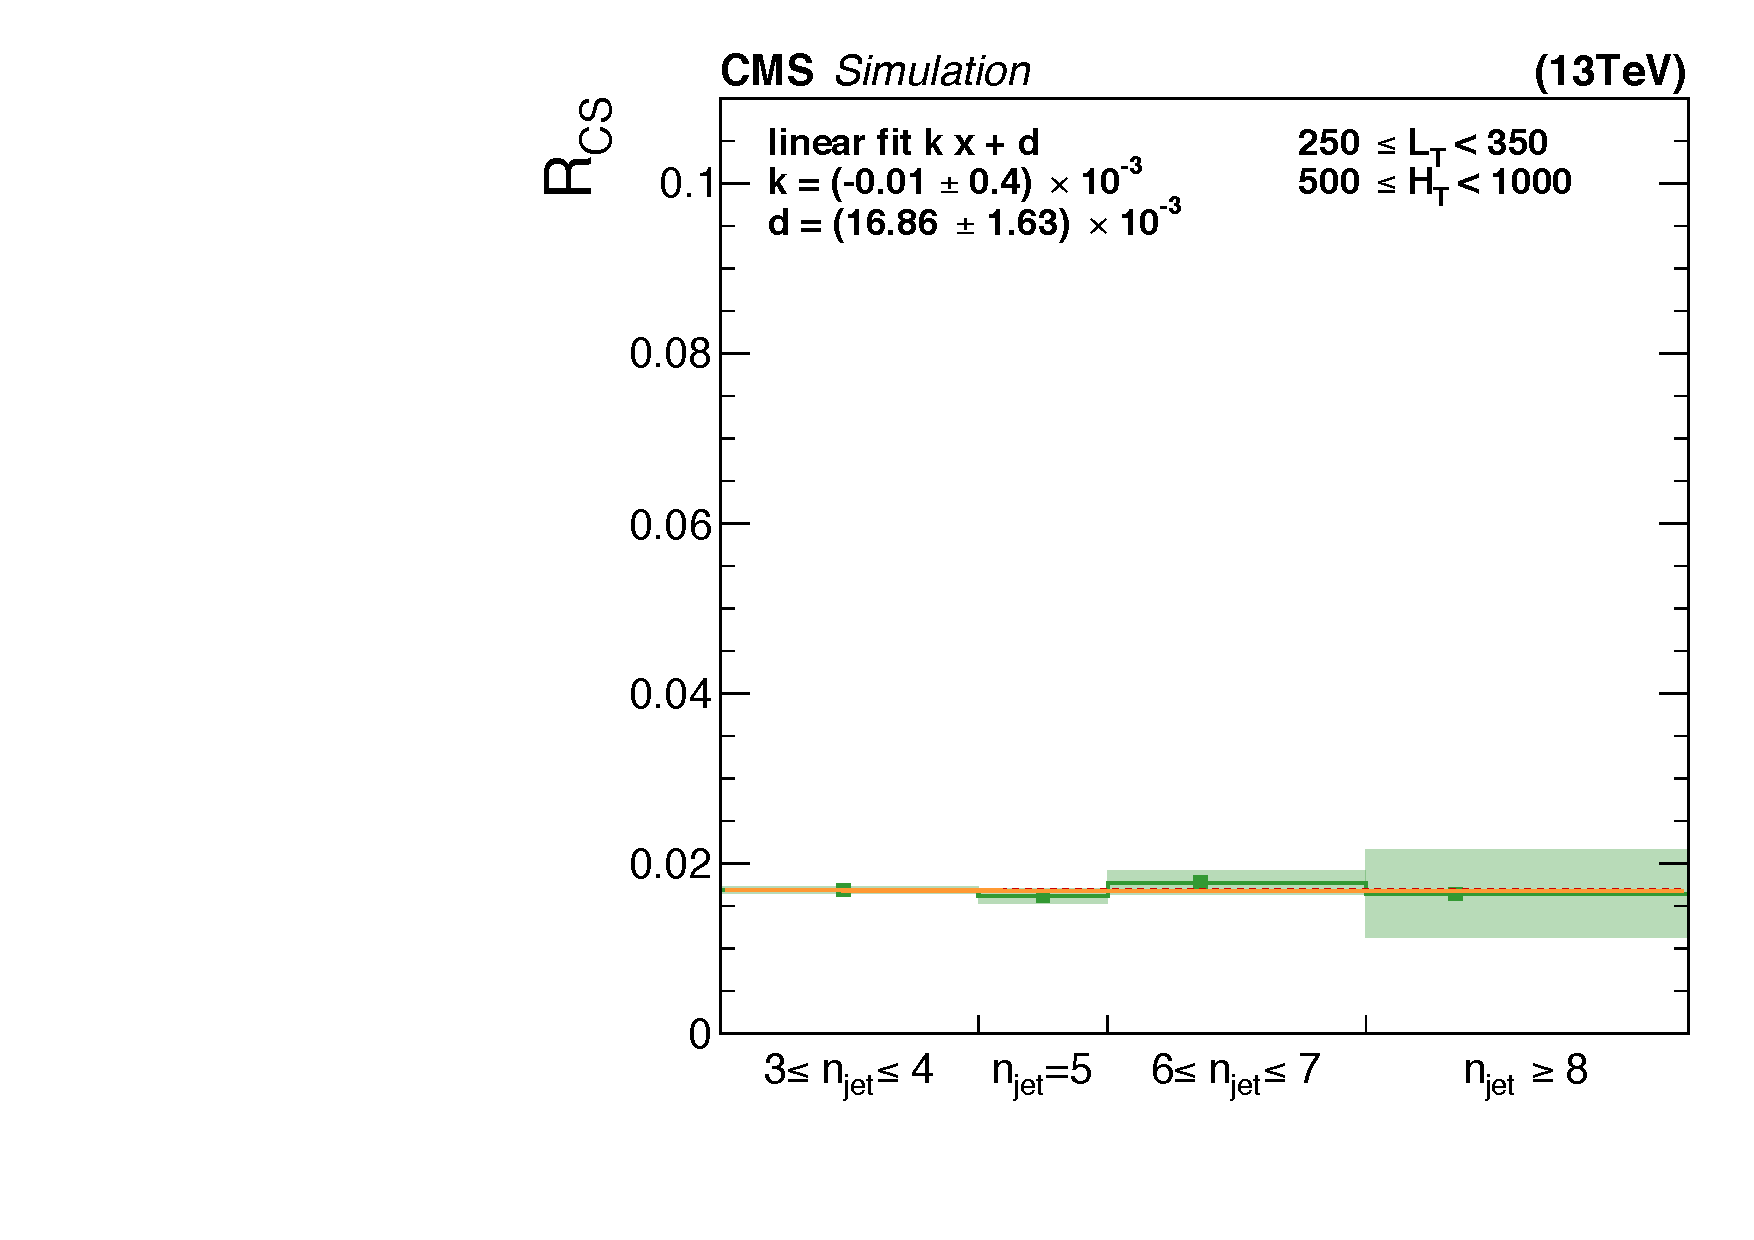
\includegraphics[width=0.45 \textwidth]{Plots/analysis/RCS/st250-350_ht500-1000_njet8_nbtag0_Wjets_NegPdg_fit}
% 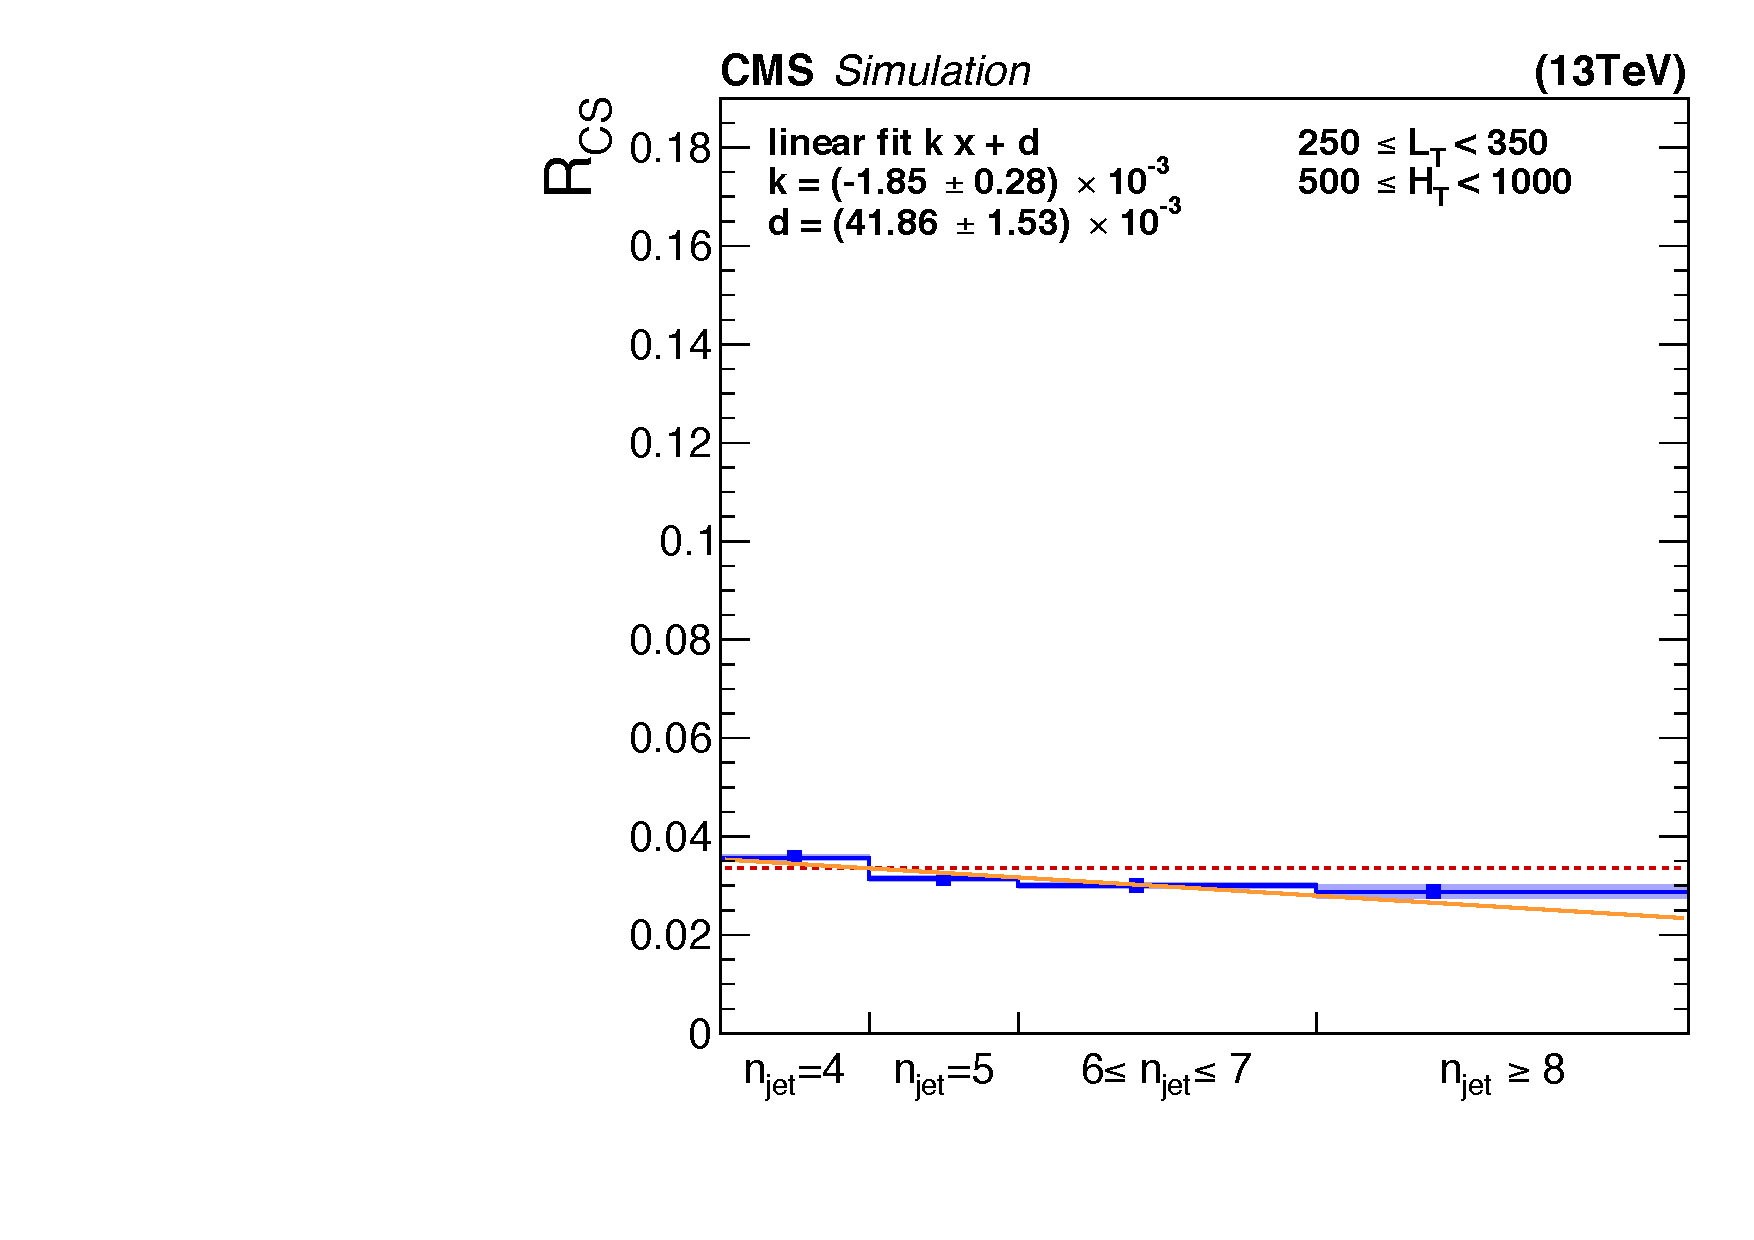
\includegraphics[width=0.45 \textwidth]{Plots/analysis/RCS/st250-350_ht500-1000_njet8_nbtag0_ttjets_all_fit}
%  \caption{ \label{fig:rcsMC} $\Rcs$ distributions as a function of $\njet$ for $\wJets$ (left) and $\ttJets$ (right) simulated events. Distributions belong to $\LT$ [250,350] GeV , $\HT$ [500,1000] GeV bin. 
% }
%  \end{center}
%\end{figure*}
%Residual differences between the $\Rcs$ in the SM and MB is calculated in simulation as a correction factor $\kappa$. Then, the predicted event counts are  corrected with this factor. For this analysis, two $\kappa$ factors for $\wJets$ and $\ttJets$ are evaluated and these will be explained in the following dedicated sections. 
%The QCD multijet background is estimated in a fake-lepton enriched data sample and it is introduced in section \ref{sec:QCDest}.  
\section{QCD background estimation}
\label{sec:QCDest}
Due to the complicated nature of quantum chromodynamics (see Sec.~\ref{sec:StandardModelParticleInteractions}), simulation of QCD multijet events is challenging and often fails to be accurate. In such a case, a data-driven prediction of the QCD multijet contribution is necessary.
According to simulation, the majority of the QCD multijet events are located in CRs and side band (low $\njet$) regions.
Although, QCD multijet events are not one of the main backgrounds, their contamination needs to be subtracted from the SBs and CRs of MBs.\\
Contributions from QCD multijet to signal region occur when a jet is misidentified as a lepton~(fake lepton). The QCD multijet contamination is negligible in the after single muon selection, therefore, the prediction is only performed in single electron events. A control sample enriched with fake electrons is obtained by inverting the criteria on lepton identification variables~(see Sec.~\ref{sec:PFelectrons}). These anti-selected electrons are required to fail the tight criteria in Tab.~\ref{tab:eleId}, but are still required to satisfy the loose electron Id.
Additionally, H/E is required to exceed 0.01 and the requirements on the IP parameters $\rm d_{xy}$ and $\rm d_z$ as well as the photon conversion veto are removed. The isolation observable $\rm I_{mini}$ is required to be below 0.4, in contrast to 0.1 for the tight electron selection.\\
To estimate the fraction of events with fake leptons, that pass the analysis selection, ratio of selected to anti-selected events ($F_{\rm sel}$) is used. To ensure the orthogonality to the mainband regions, this ratio is measured in the $3\leq\njet\leq4$ and $\nbjet=0$ sideband.\\
The kinematic properties of the fake leptons helps to distinguish QCD~multijet events from the EWK ones (containing prompt electrons) by using a variable which reflects the polarization of the W boson. The variable $\LP$ was introduced in~\cite{LP}, and was used for the first measurement of the W polarization at LHC.
The variable $\LP$ is defined:
\begin{equation}
\label{eq:LP}
{\LP} = \frac{\ptvec(\ell)\cdot\ptvec(W)}{|\ptvec(W)|^2} = \frac{\pt(\ell)}{\pt(W)} \rm cos(\DF(W,\ell)),
\end{equation}
where $\pt(\ell)$ and $\pt(W)$ are the transverse momenta of the charged lepton and the W boson respectively.\\
As seen in Fig.~\ref{fig:QCD}, QCD multijet events~(dashed cyan colored lines) mostly populate the $\LP$ close to 1 while the EWK events have a falling distribution from 0 to 1. The number of QCD multijet events in the control regions for selected leptons is then obtained by multiplying the yield of the anti-selected events, which is obtained from the example template fit shown in Fig.~\ref{fig:QCD}~(left), with $F_{\rm sel}$ which is shown right, as a function of $\LT$.\\
A profound description of the method can be found in~\cite{David}.
\begin{figure*}[!hbt]
    \begin{center}
 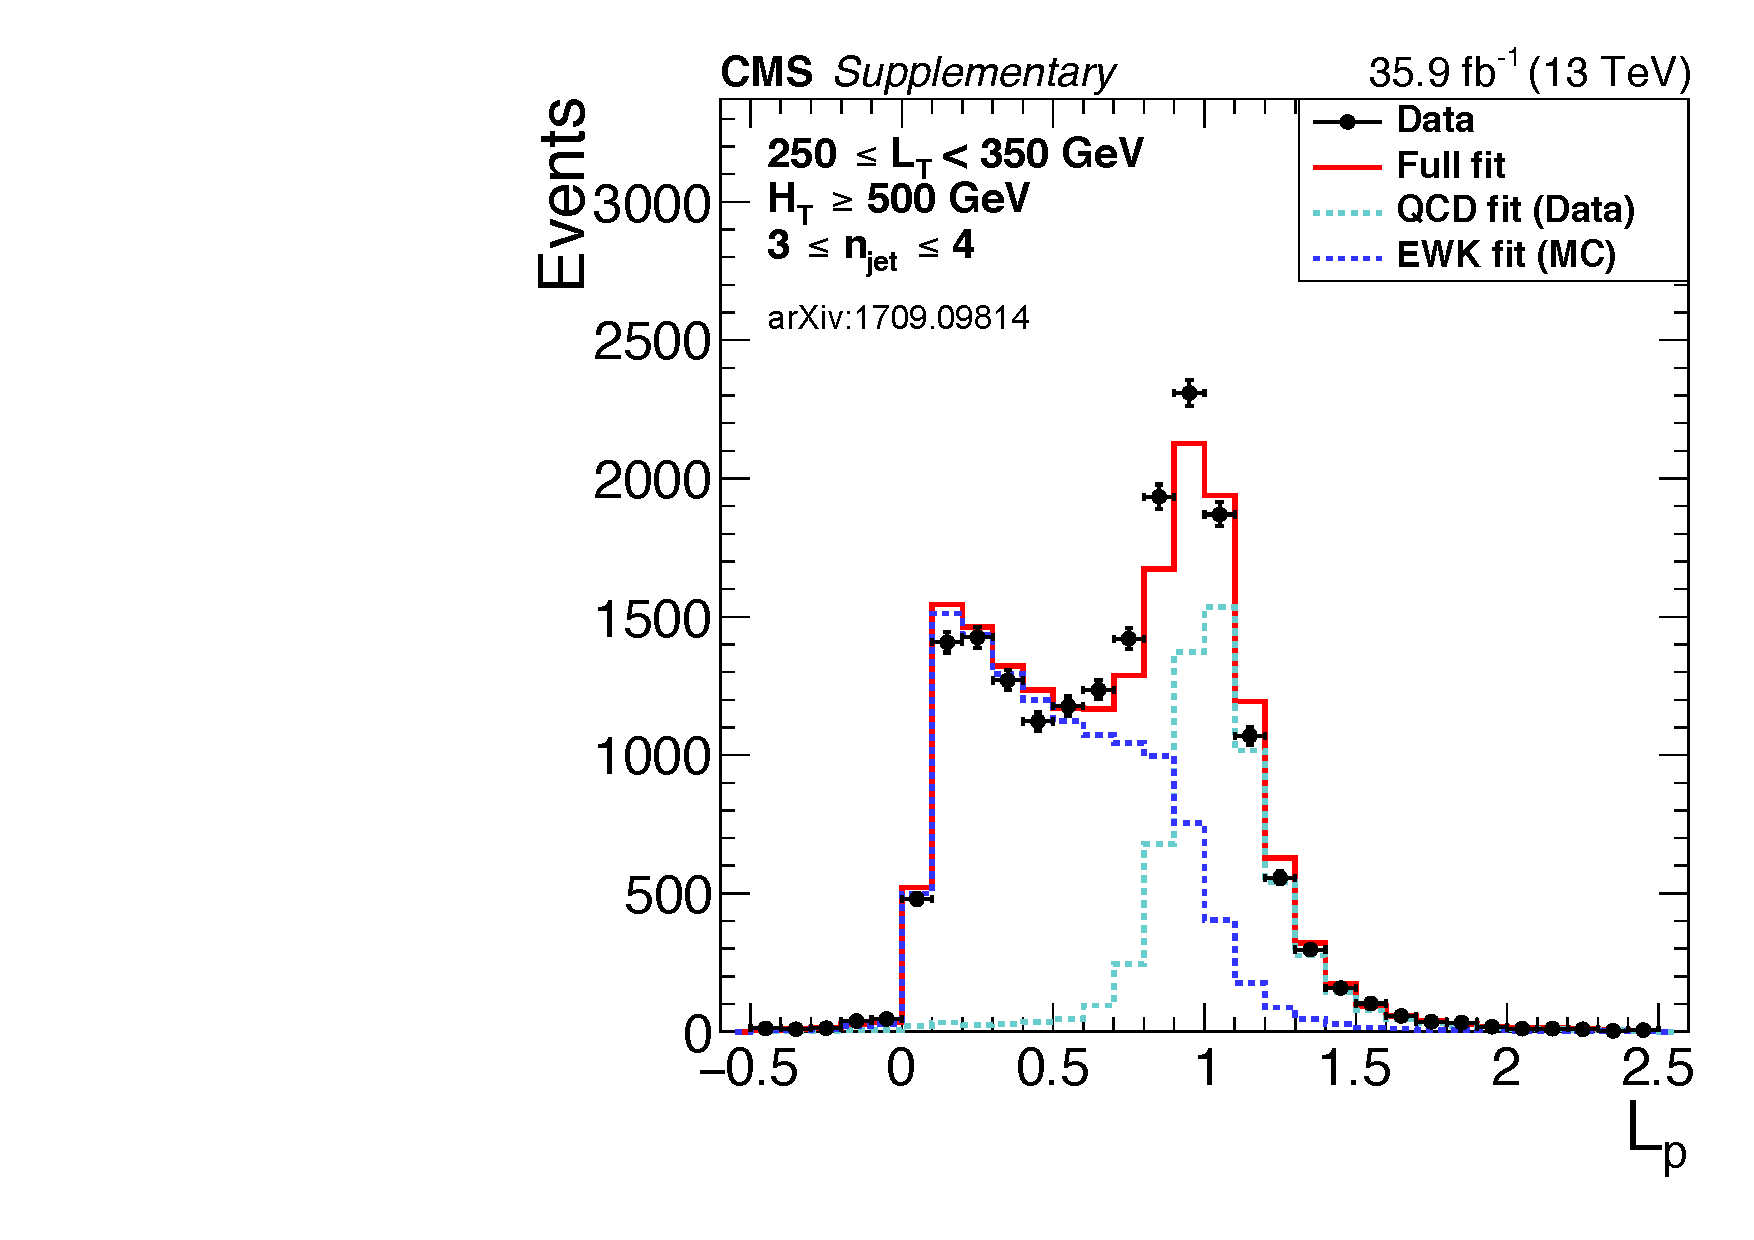
\includegraphics[width=0.45 \textwidth]{PhD_Thesis_v4/Plots/analysis/QCD/QCD_Lp_singleElectronic_st250-350_ht500_njet3-4_nbtagEq0_TemplateFit.pdf}
 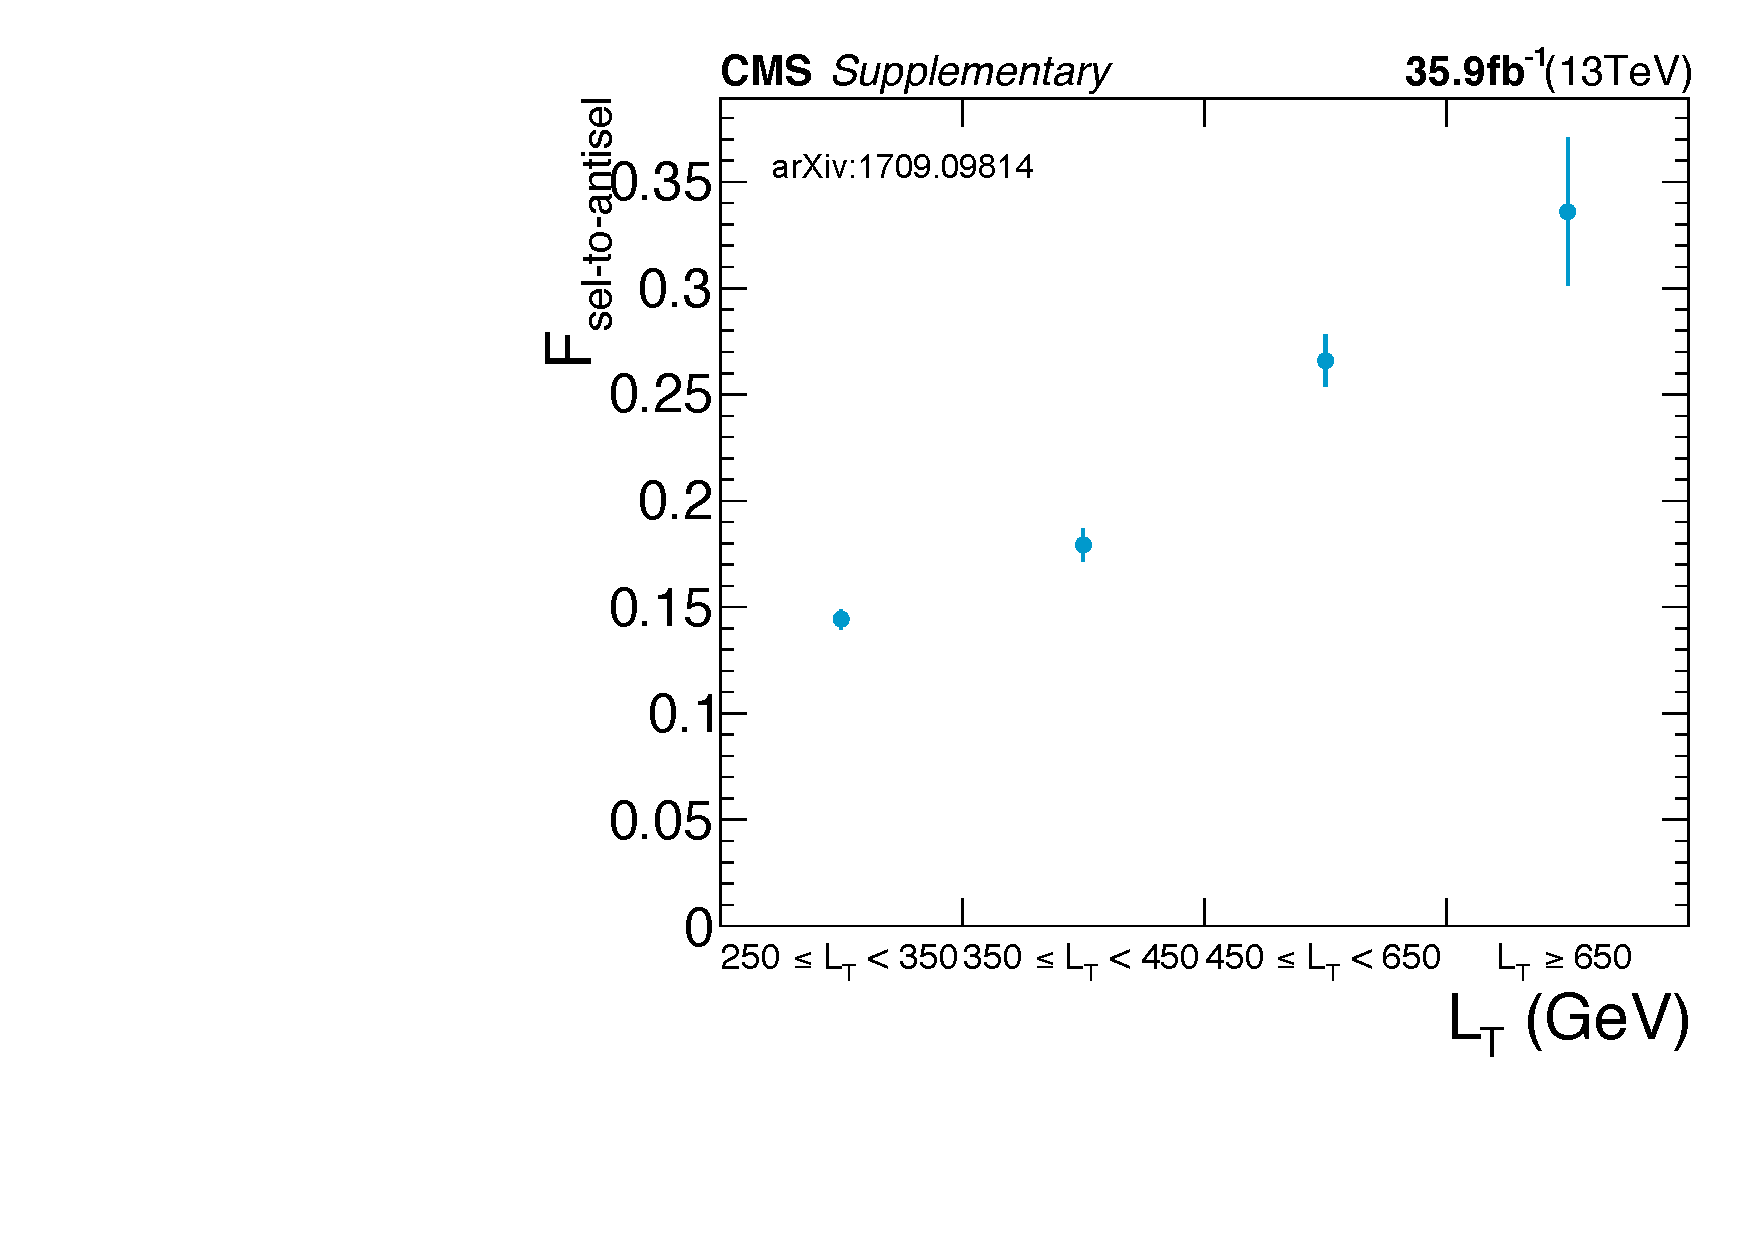
\includegraphics[width=0.45 \textwidth]{PhD_Thesis_v4/Plots/analysis/QCD/QCD_Fsel.pdf}
  \caption{ \label{fig:QCD} The $\LP$ shape fit result for $3\leq\njet\leq4$ and $\nbjet=0$ in the $250\leq\LT\leq350$ bin (left).  Ratio of selected to anti-selected electron events from QCD multijet events for $3\leq\njet\leq4$ and $\nbjet=0$, in bins of LT in data (right). 
 }
  \end{center}
\end{figure*}
\section{Background fraction calculations: b-tag multiplicity fit}
\label{sec:bkgcomp}
Fractions of the background processes in the control regions ($f^{CR}_i$) are calculated using a likelihood fit of b-tag multiplicity distribution templates to data. The templates are obtained from simulation, with the exception of QCD multijet events. The latter contribution is taken from the data driven prediction which is described in Sec.~\ref{sec:QCDest}.
$\wJets$ events are not produced symmetrically in lepton charge at a pp collider. To account for this, the fits are performed separately for the positive and negative lepton charge. The $\ttJets$ and QCD multijet contribution is assumed to be symmetric. Other background templates are also produced separately for positive and negative charged leptons. 
Fig.~\ref{fig:btagmult} shows data~(black points) and the b~tag multiplicity fit~(blue dashed line).
\begin{figure*}[!hbt]
    \begin{center}
 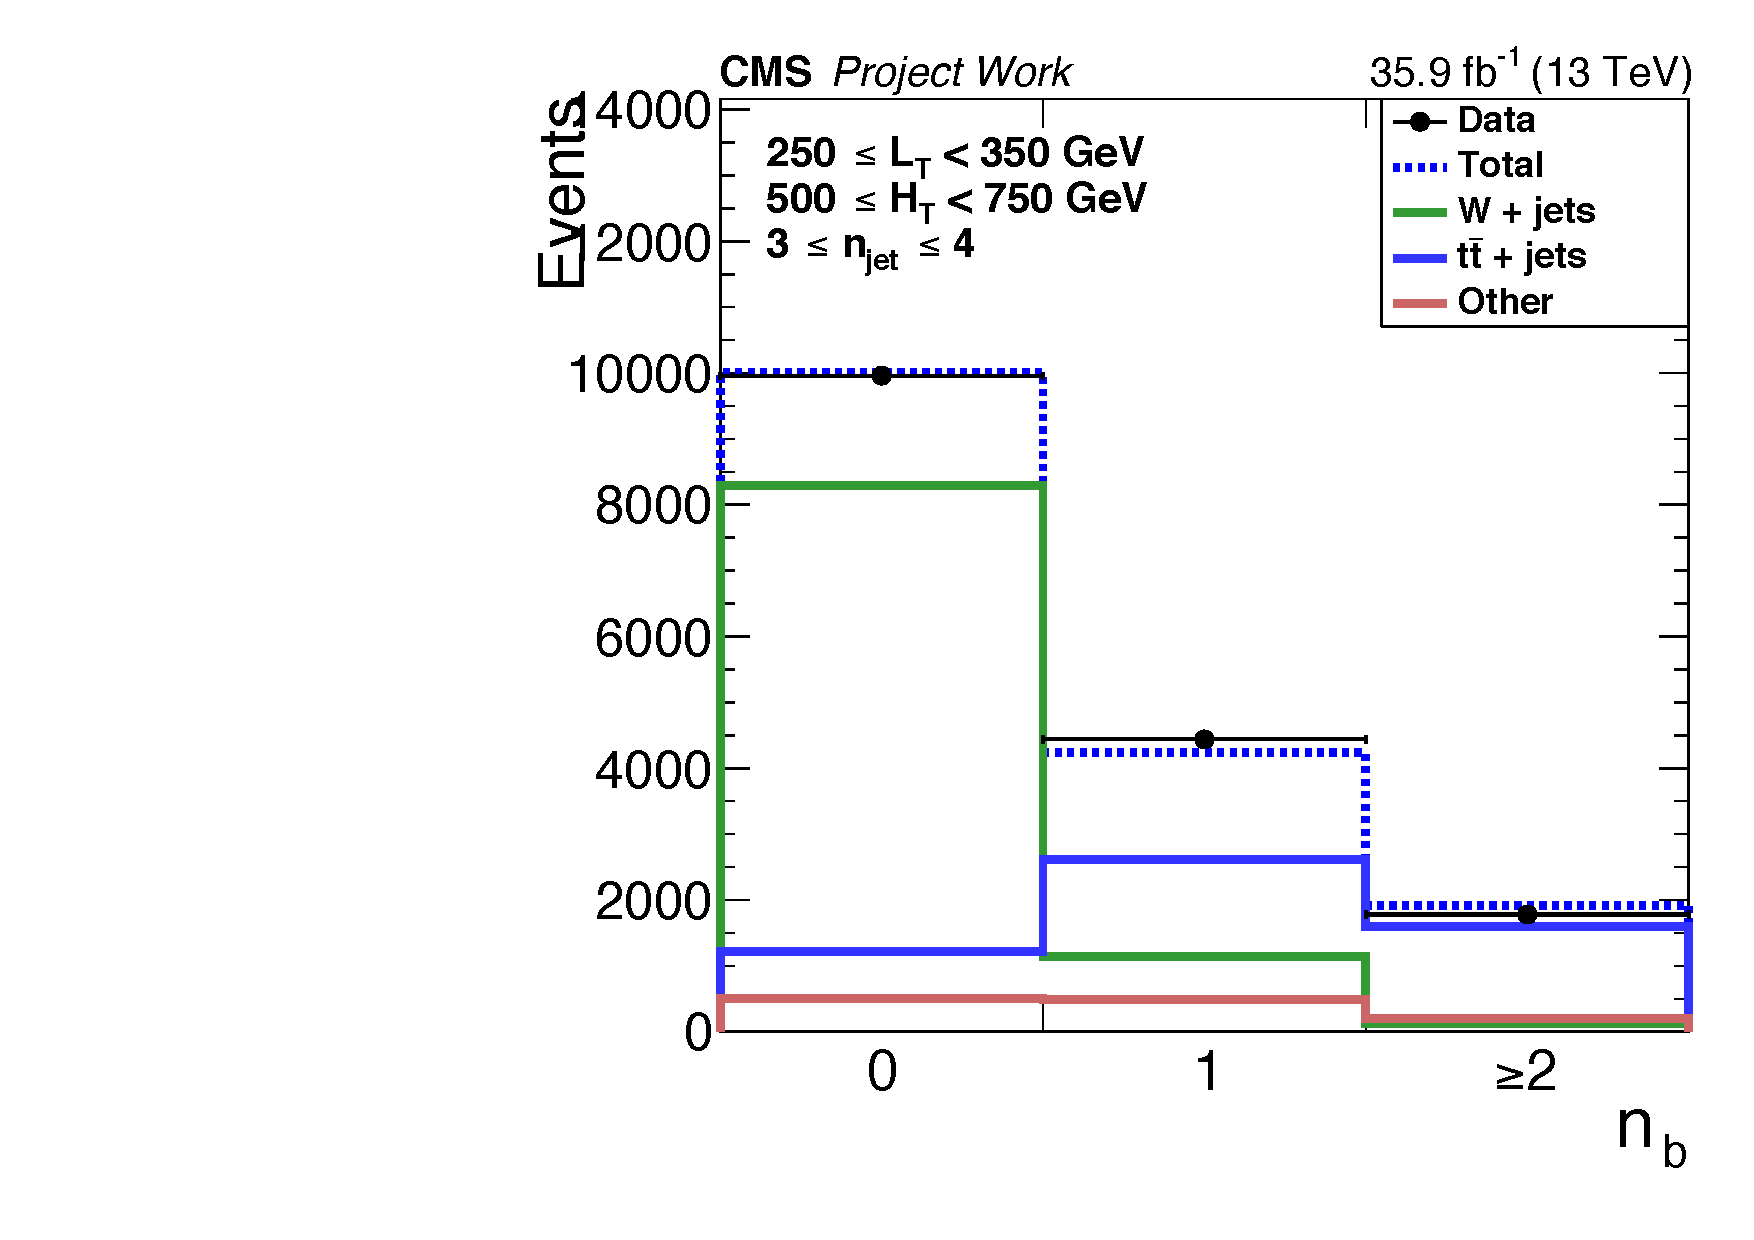
\includegraphics[width=0.48 \textwidth]{PhD_Thesis_v4/Plots/analysis/RCS/btagfits/st250-350_ht500-750_njet3-4_nBTagFitRes.pdf}
 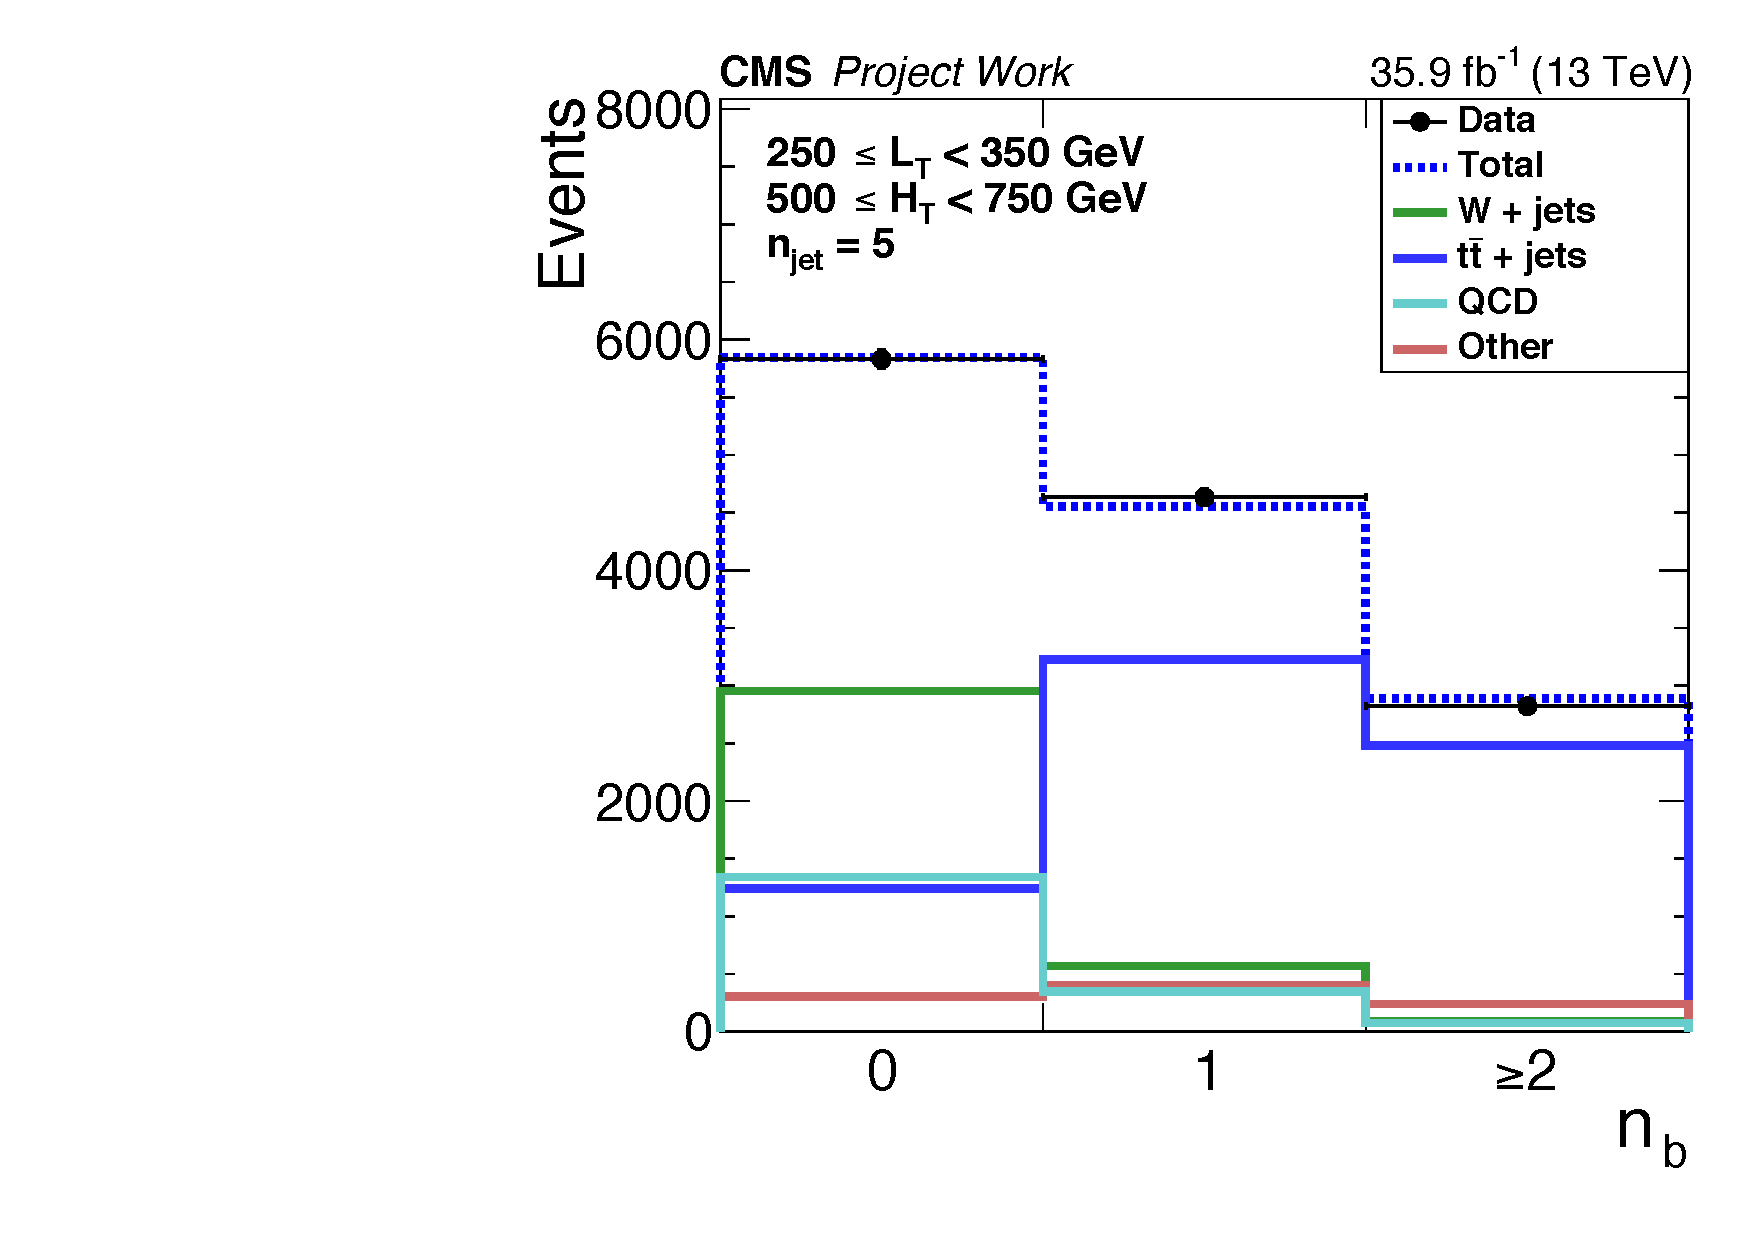
\includegraphics[width=0.48\textwidth]{PhD_Thesis_v4/Plots/analysis/RCS/btagfits/st250-350_ht500-750_njetEq5_nBTagFitRes.pdf}\\
  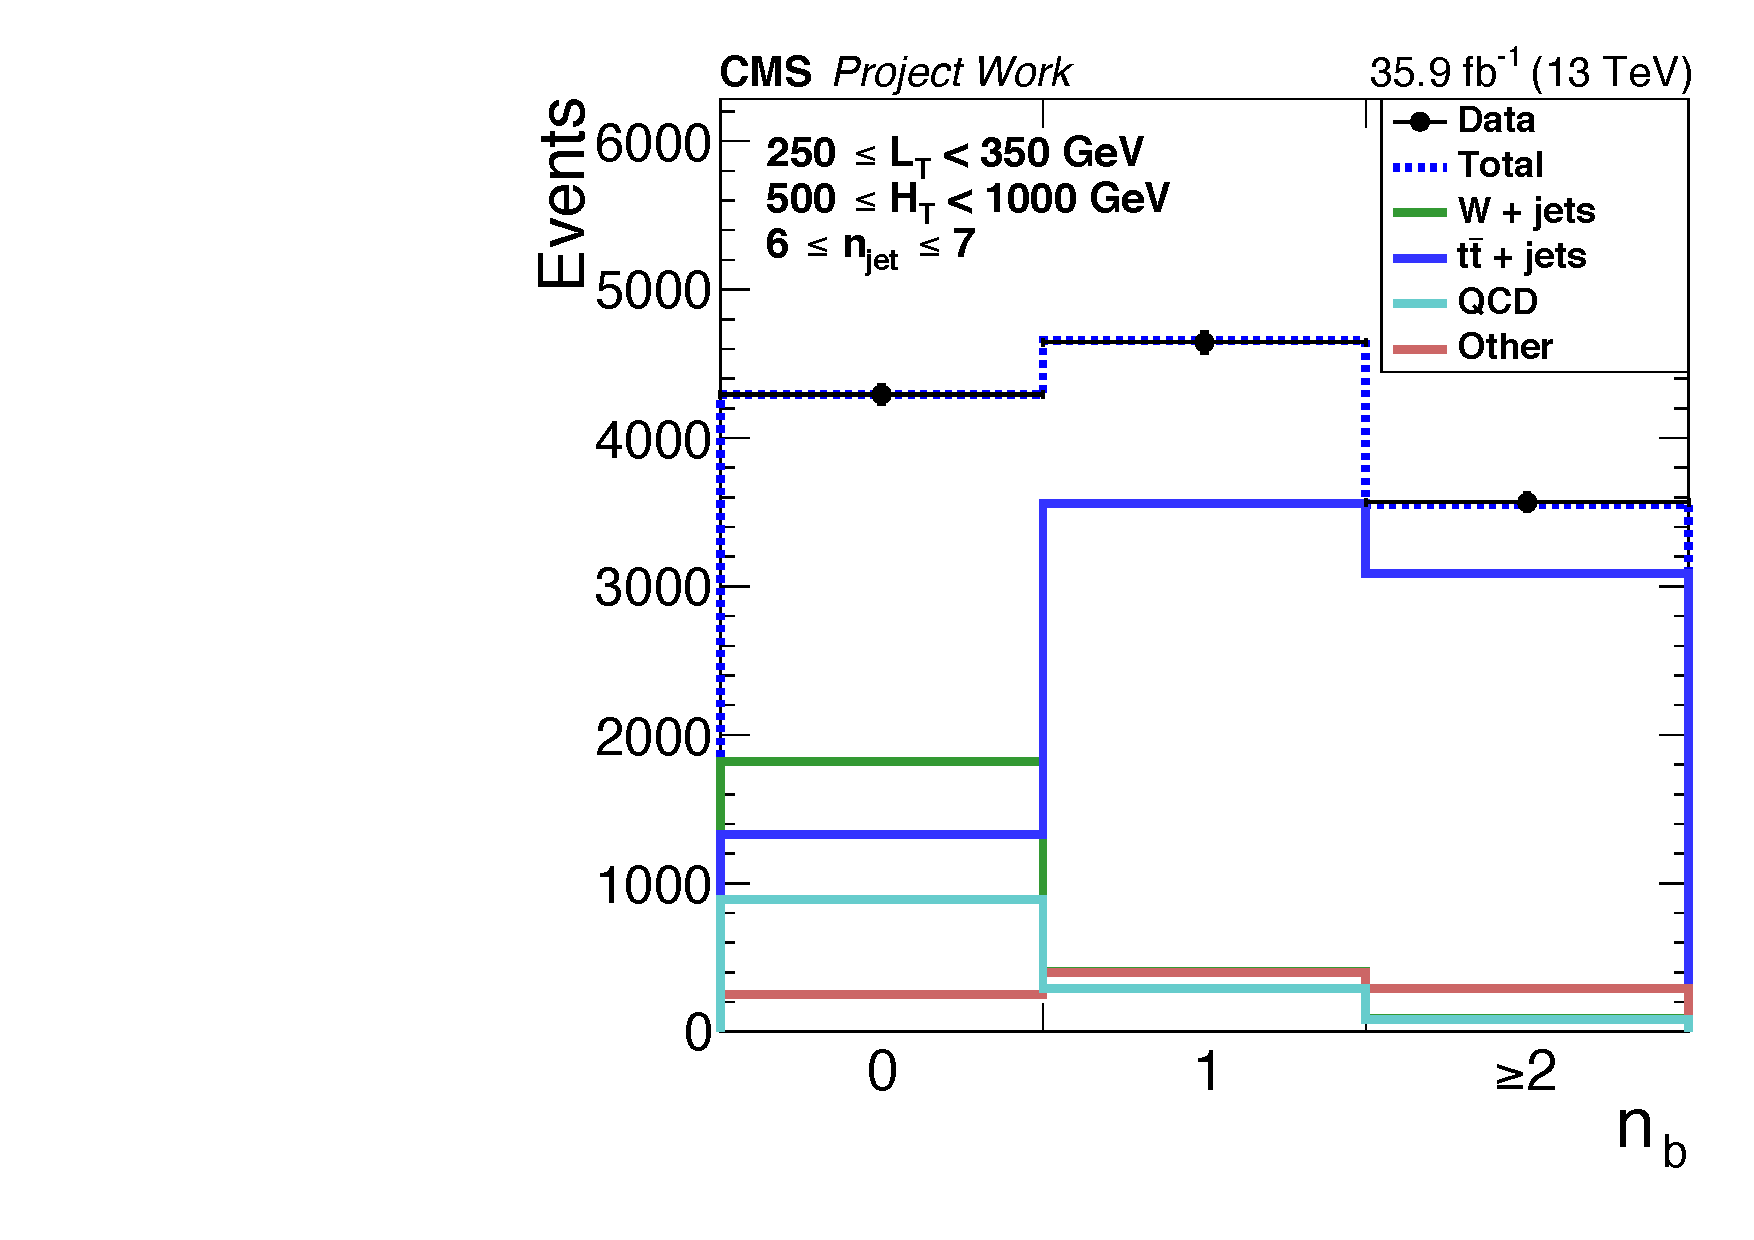
\includegraphics[width=0.48 \textwidth]{PhD_Thesis_v4/Plots/analysis/RCS/btagfits/st250-350_ht500-1000_njet6-7_nBTagFitRes.pdf}
 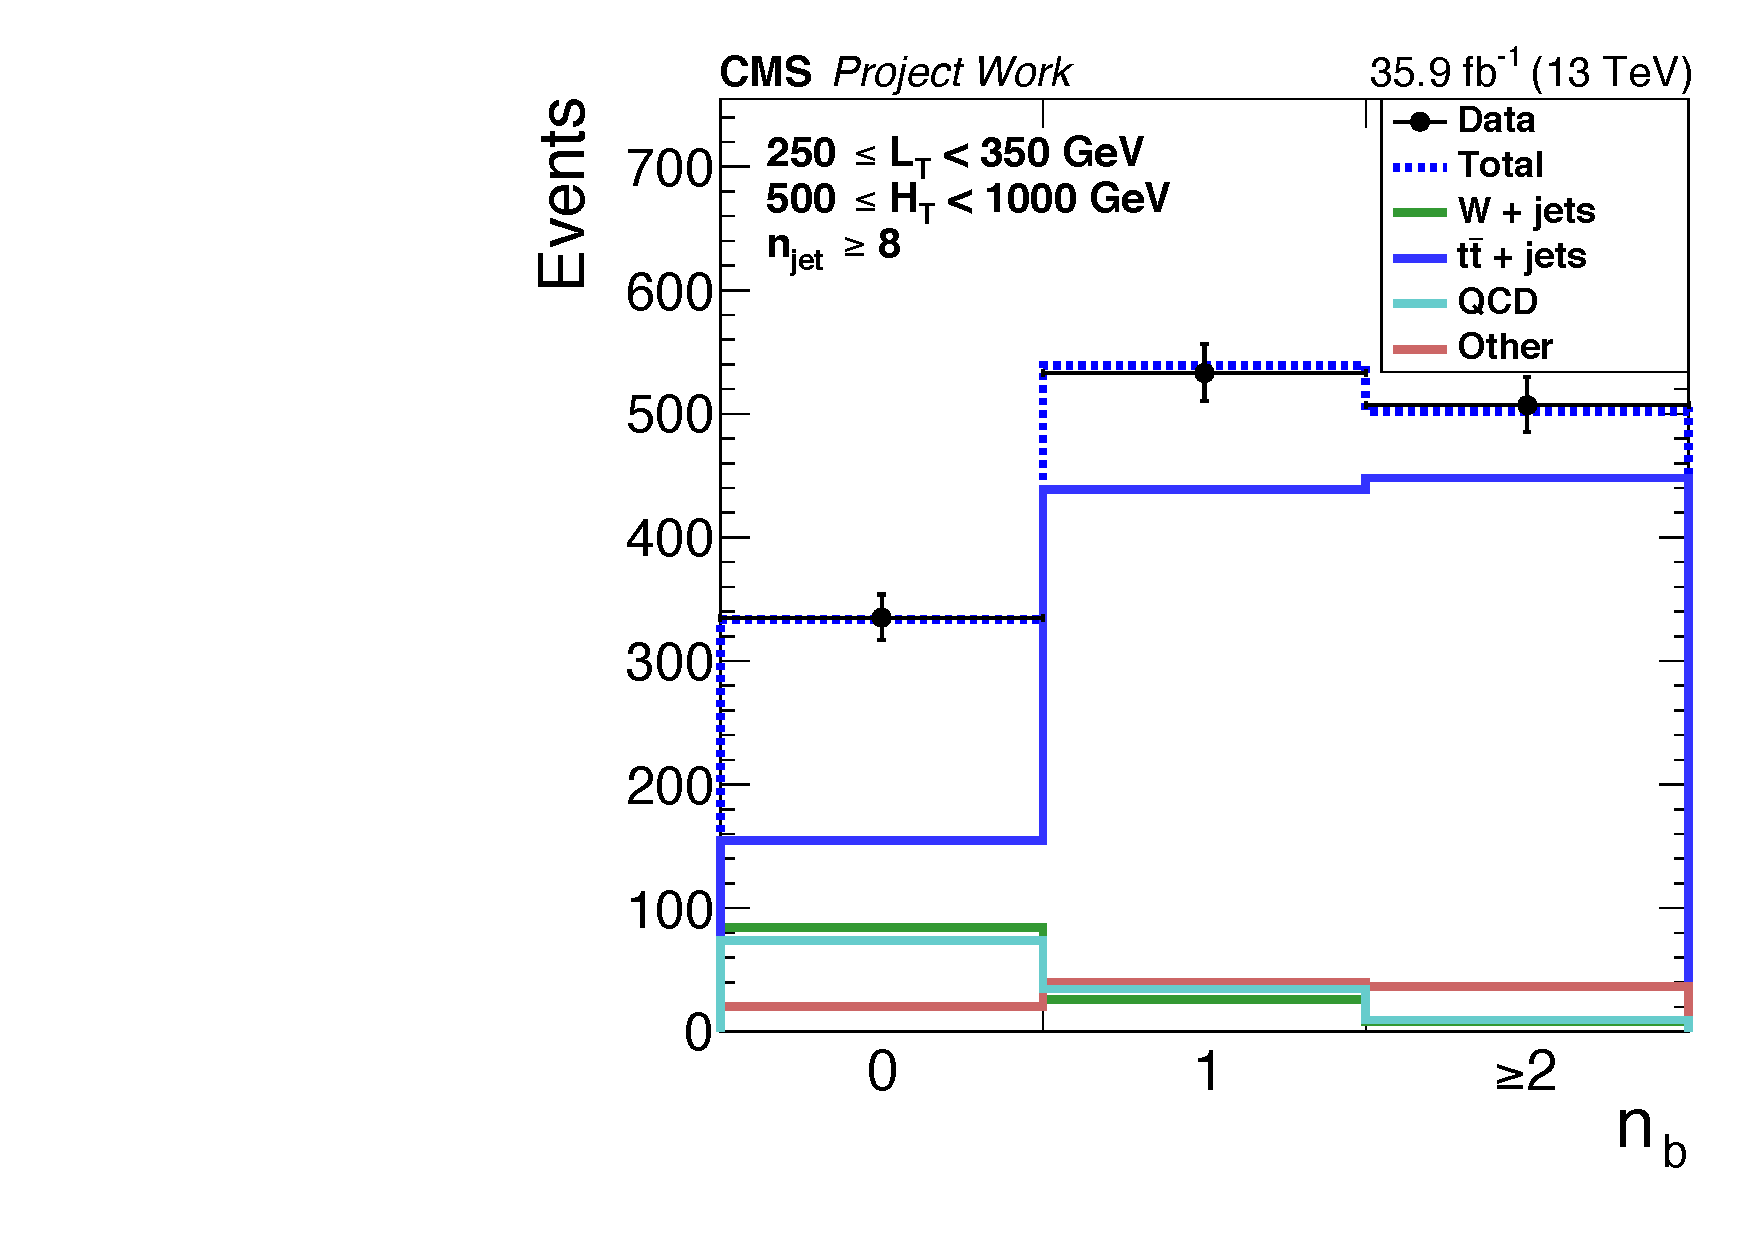
\includegraphics[width=0.48\textwidth]{PhD_Thesis_v4/Plots/analysis/RCS/btagfits/st250-350_ht500-1000_njet8_nBTagFitRes.pdf}
  \caption[The b-tag multiplicity fit examples]{ \label{fig:btagmult} b-tag multiplicity fit is performed in control regions. 3-4 jets sideband (top/left), 5 jets mainband (right/top), 6-7 jets mainband (left/bottom) and 8 or more jets mainband fits are shown. Black points represent data, green is for $\wJets$ , blue is for $\ttJets$ , orange is for other EWK backgrounds and  cyan colored lines show QCD contamination.
 }
  \end{center}
\end{figure*}
\section{$R_{CS}$ method in $\ttJets$ events}
\label{sec:RcsTT}
At the LHC, the top quark pair production mechanism is dominated by gluon-gluon fusion~(80\%) and quark-quark annihilation(20\%). According to the SM, the top quark decays into W and b quark in almost 100\% of the cases\footnote{CKM induced flavour violating decays are neglected in this thesis}, thus predicting two b quark partons in the tt+jets final state. However, the b tagging algorithms are not fully efficient; therefore $\ttbar$ events can survive veto on b-tagged jets. The remaining events have a very similar final state as the T5qqqqWW signal events.\\
%Due to its high cross section,  $\ttJets$ is one of the two main backgrounds. \\
The $\ttbar$ decay can be split in three categories according to the lepton content of the final state; single leptonic, dileptonic and fully hadronic. The branching ratios of these decay modes are 43.8\%, 10.5\% and 45.7\%, respectively.  After the baseline selection, the single leptonic decay channel, where one of the two W bosons decays leptonically, populates the low $\DF$ region while the dileptonic decay channel, where one of the leptons is lost to misidentification or the limited detector acceptance, dominates the high $\DF$ region. As a result of the induced $\MET$, the dileptonic $\ttbar$ contribution can have high $\Rcs$ values. For illustration, Fig.~\ref{rcsMCtt} shows the simulated $\Rcs$ as a function of $\njet$ for dileptonic (left) and single leptonic (right) decays separately.
\begin{figure*}[!hbt]
    \begin{center}
 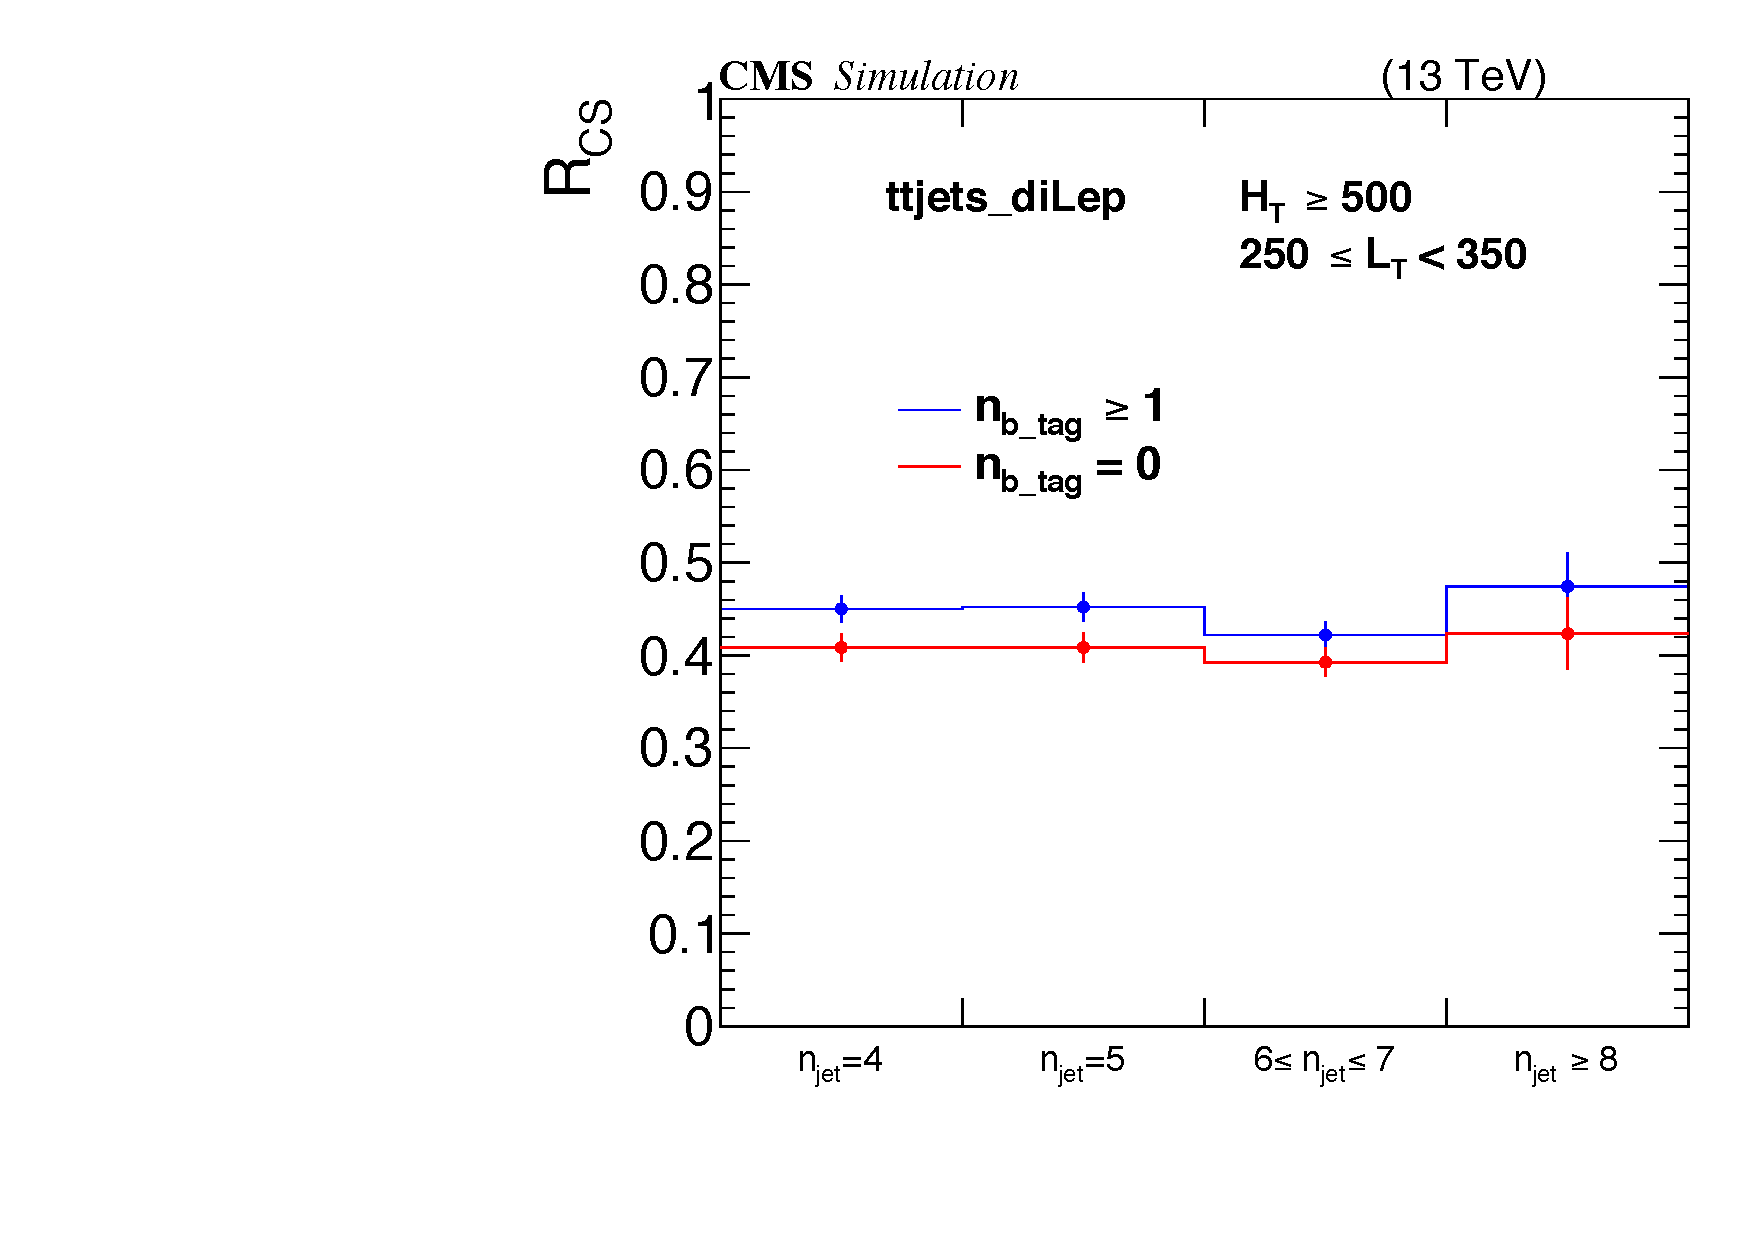
\includegraphics[width=0.45 \textwidth]{Plots/analysis/RCS/dilep}
    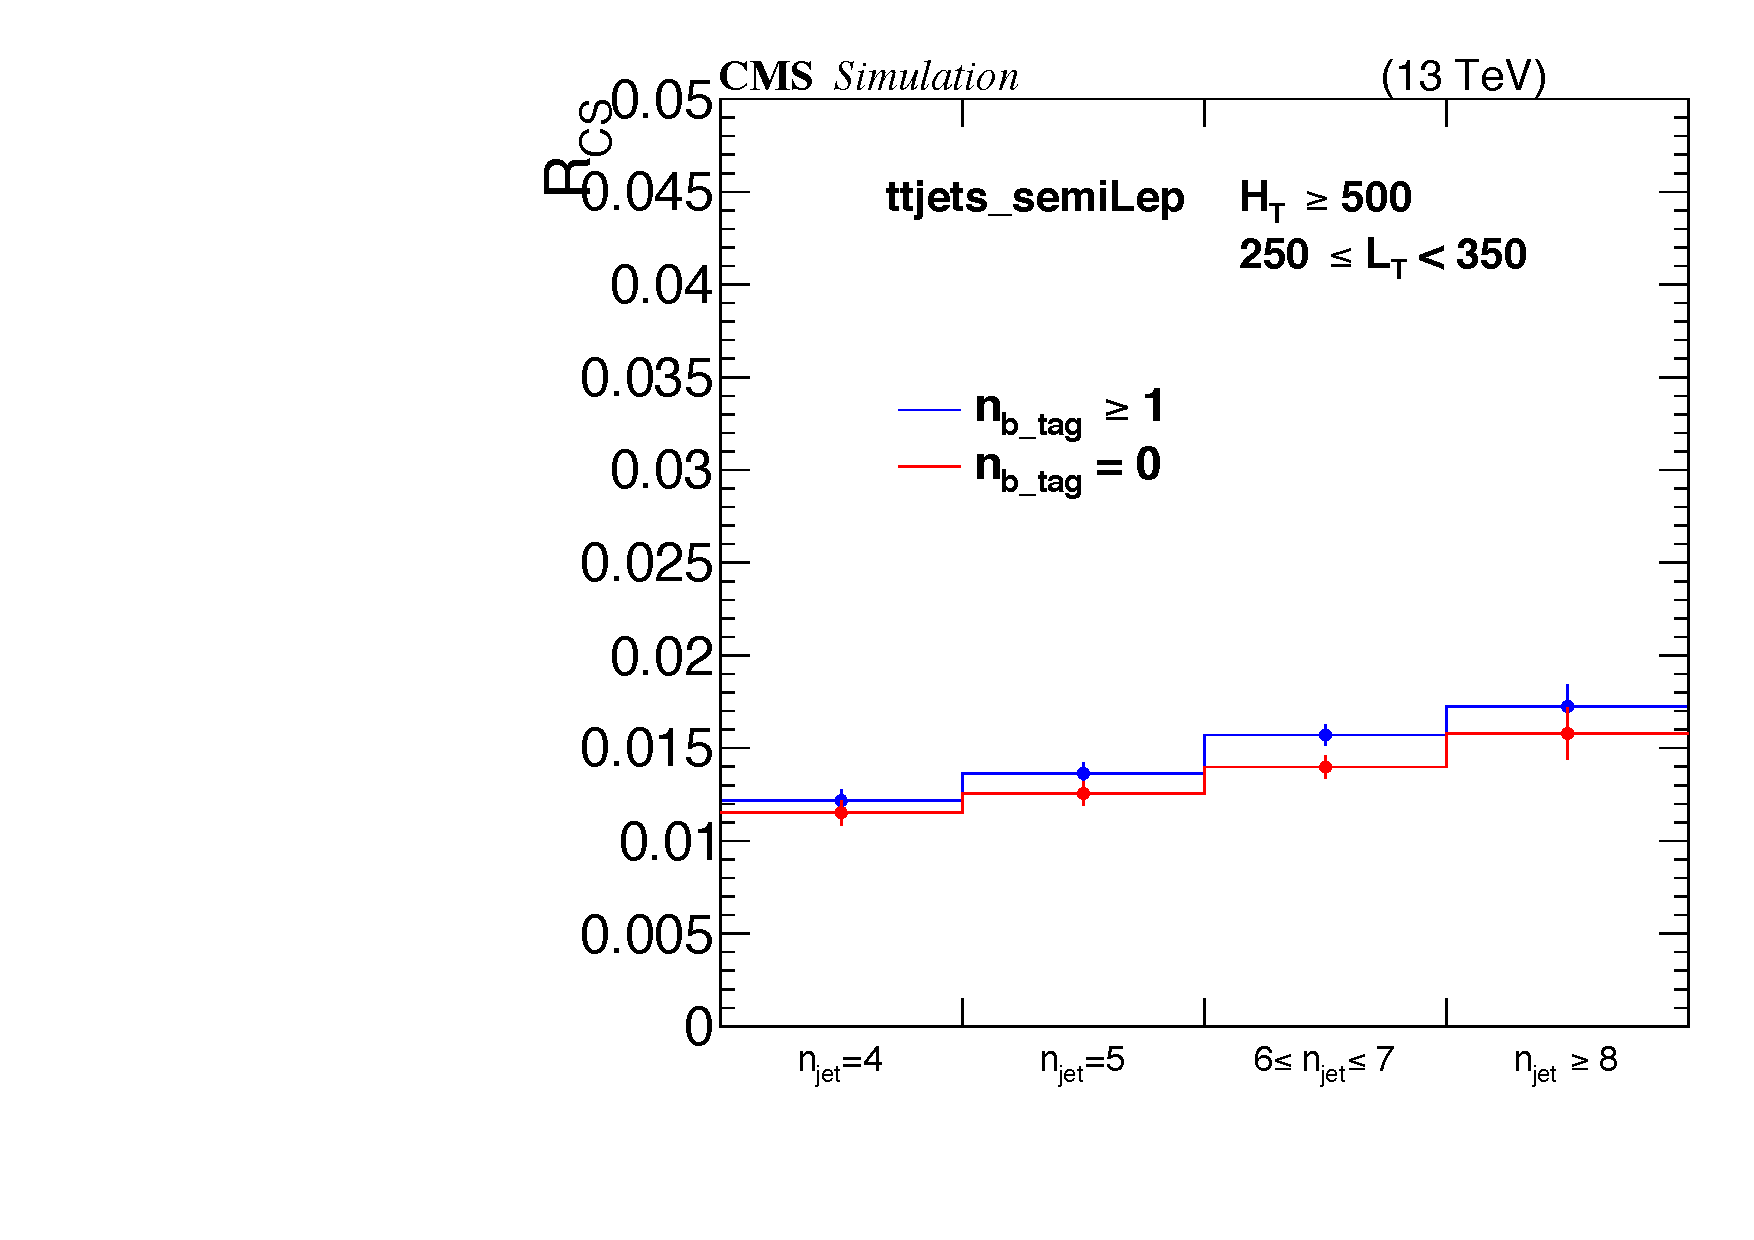
\includegraphics[width=0.45 \textwidth]{Plots/analysis/RCS/semilep}
  \caption{ \label{rcsMCtt}  $\Rcs$ as a function of njet for dileptonic (left), and single leptonic (right) tt + jets events. }
  \end{center}
\end{figure*}
In the primary background estimation procedure, $\Rcs$ values of $\ttJets$ yields are measured in data sideband regions, requiring four to five jets and at least one b-tagged jet. This selection increases the purity of $\ttJets$ events and keeps the $\wJets$ contamination low. In addition to this, the yield of predicted QCD multijet events is subtracted from the CR, in summary:
\begin{equation}
\label{eq:rcsTTdata}
\Rcs^{data}(b \geq 1, \njet \in [4,5] ) = \frac{N_{SR}^{data}}{N_{CR}^{data}-N_{CR}^{QCD(pred)}}.
\end{equation}
Figure~\ref{RCS_dataMCtt} shows the simulated $\Rcs$ in low $\HT$~(left), and high $\HT$~(right) values for the first search bin which is $\njet =$~5, $\LT \in$~[250,350]~GeV. The simulated and measured $\Rcs$ values are shown in Tab.~\ref{tab:rcsTTcomp}.\\
Residual differences between $\Rcs$ in the sideband and mainband are obtained in simulation as a correction factor $\kappa$. In $\ttJets$ background estimation, $\kappa=\kappa_b\cdot\kappa_{\ttbar}$.
\begin{figure*}[!hbt]
    \begin{center}
 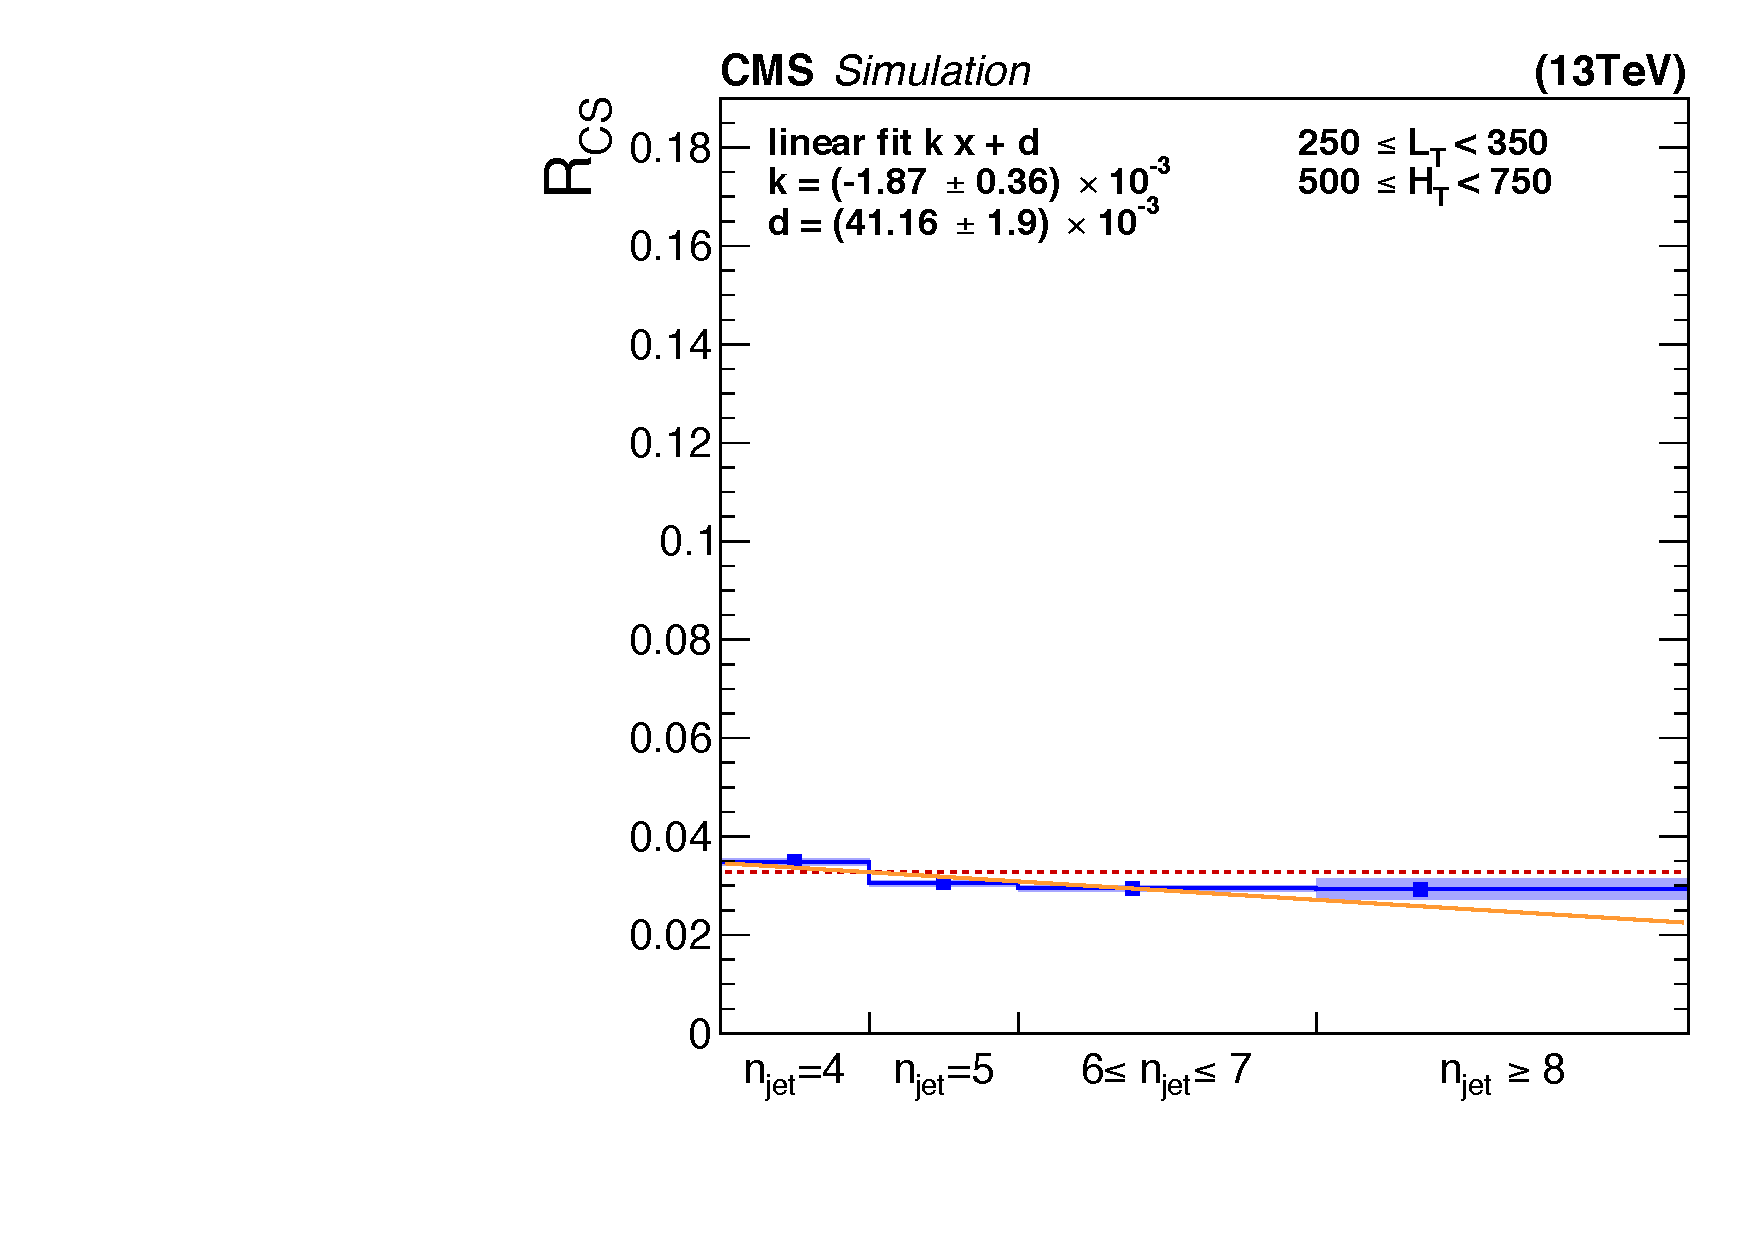
\includegraphics[width=0.45 \textwidth]{PhD_Thesis_v4/Plots/analysis/RCS/st250-350_ht500-750_njet8_nbtag0_ttjets_all_fit.pdf}
    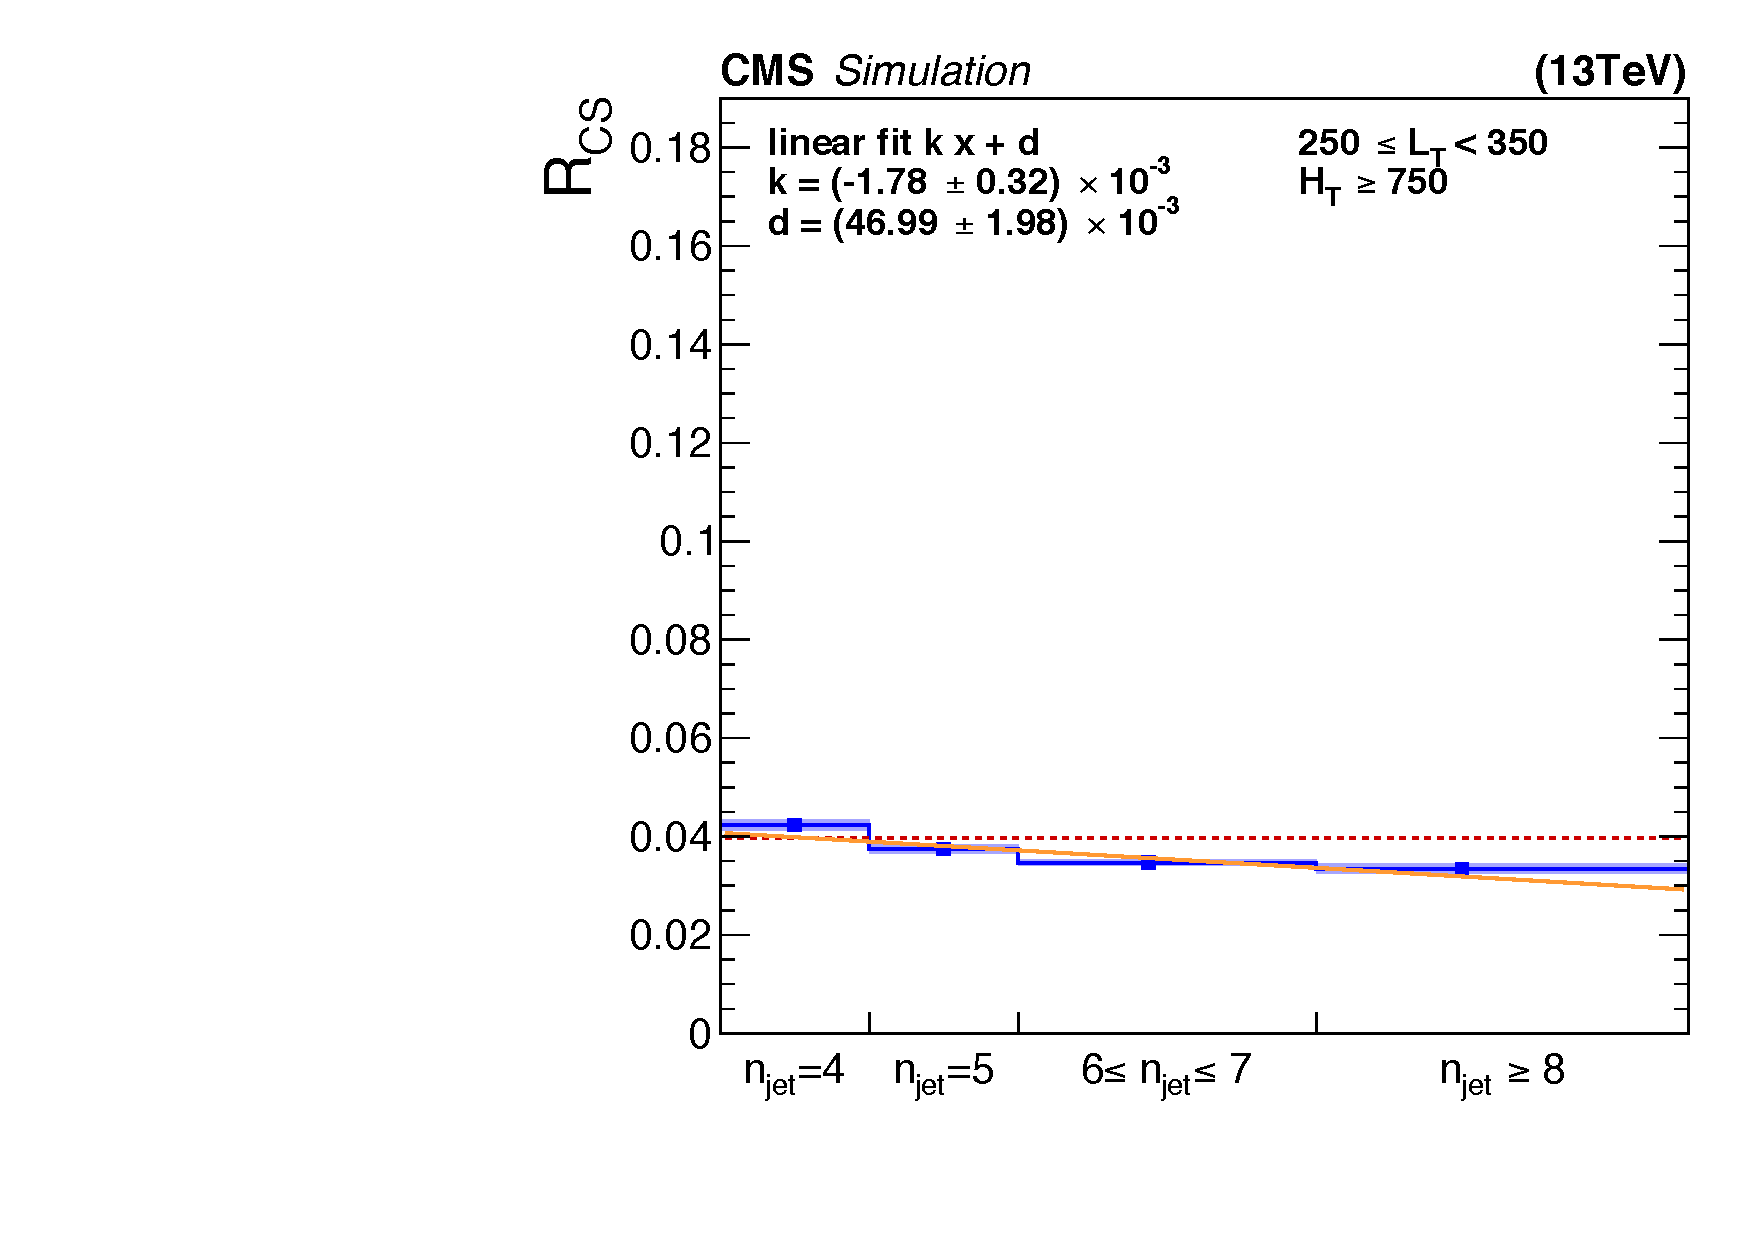
\includegraphics[width=0.45 \textwidth]{PhD_Thesis_v4/Plots/analysis/RCS/st250-350_ht750_njet8_nbtag0_ttjets_all_fit.pdf}
  \caption{ \label{RCS_dataMCtt}  The factor $\Rcs$ as a function of $\njet$ from simulation of $\ttJets$ events for low $\HT$~(left), and high $\HT$~(right). The red line shows the $\RCS$ value in the SB that is 4-5j, b$\geq$1. The difference between the linear fit and the red line is used to measure systematic uncertainty.}
  \end{center}
\end{figure*}
\begin{table}[ht]\begin{center}
\caption{Simulated and measured $\Rcs$ of the $\ttJets$ events.\label{tab:rcsTTcomp}}
\resizebox{\textwidth}{!}{\begin{tabular}{|c|c|c|rrr|rrr|}\hline
 \multirow{2}{*}{\njet}     & \LT       & \HT & \multicolumn{6}{c|}{$\Rcs$ in 4-5j, $\geq$1b}\\%\hline
 & $[$GeV$]$                 &$[$GeV$]$ &\multicolumn{3}{c|}{simulated} &\multicolumn{3}{c|}{measured}                     \\\hline
\hline
\multirow{10}{*}{\begin{sideways}$5$\end{sideways}}
&\multirow{2}{*}{$[250,350]$}
&$[500,750]$
 & 0.0373&$\pm$&0.0005& 0.0413&$\pm$&0.0017
 \\
&
&$\geq750$
 & 0.0454&$\pm$&0.0008& 0.0549&$\pm$&0.0035
 \\
\cline{2-9}
&\multirow{2}{*}{$[350,450]$}
&$[500,750]$
 & 0.0265&$\pm$&0.0007& 0.0303&$\pm$&0.0026
 \\
&
&$\geq750$
 & 0.0314&$\pm$&0.0009& 0.0319&$\pm$&0.0038
 \\
\cline{2-9}
&\multirow{3}{*}{$[450,650]$}
&$[500,750]$
 & 0.0375&$\pm$&0.0015& 0.0359&$\pm$&0.005
 \\
&
&$[750,1250]$
 & 0.0338&$\pm$&0.0012& 0.0324&$\pm$&0.0049
 \\
&
&$\geq1250$
 & 0.054&$\pm$&0.0019& 0.0403&$\pm$&0.0137
 \\
\cline{2-9}
&\multirow{3}{*}{$\geq650$}
&$[500,750]$
 & 0.282&$\pm$&0.037& 0.1967&$\pm$&0.0971
 \\
&
&$[750,1250]$
 & 0.0449&$\pm$&0.0031& 0.0476&$\pm$&0.0127
 \\
&
&$\geq1250$
 & 0.0663&$\pm$&0.0033& 0.0641&$\pm$&0.0252
 \\
\cline{2-9}
\hline
\hline
\multirow{10}{*}{\begin{sideways}$[6,7]$\end{sideways}}
&\multirow{2}{*}{$[250,350]$}
&$[500,1000]$
 & 0.0382&$\pm$&0.0004& 0.0422&$\pm$&0.0016
 \\
&
&$\geq1000$
 & 0.0536&$\pm$&0.0013& 0.0762&$\pm$&0.0076
 \\
\cline{2-9}
&\multirow{2}{*}{$[350,450]$}
&$[500,1000]$
 & 0.027&$\pm$&0.0006& 0.0291&$\pm$&0.0022
 \\
&
&$\geq1000$
 & 0.0379&$\pm$&0.0013& 0.0459&$\pm$&0.0082
 \\
\cline{2-9}
&\multirow{3}{*}{$[450,650]$}
&$[500,750]$
 & 0.0375&$\pm$&0.0015& 0.0359&$\pm$&0.005
 \\
&
&$[750,1250]$
 & 0.0338&$\pm$&0.0012& 0.0324&$\pm$&0.0049
 \\
&
&$\geq1250$
 & 0.054&$\pm$&0.0019& 0.0403&$\pm$&0.0137
 \\
\cline{2-9}
&\multirow{3}{*}{$\geq650$}
&$[500,750]$
 & 0.282&$\pm$&0.037& 0.1967&$\pm$&0.0971
 \\
&
&$[750,1250]$
 & 0.0449&$\pm$&0.0031& 0.0476&$\pm$&0.0127
 \\
&
&$\geq1250$
 & 0.0663&$\pm$&0.0033& 0.0641&$\pm$&0.0252
 \\
\cline{2-9}
\hline
\hline
\multirow{8}{*}{\begin{sideways}$\geq8$\end{sideways}}
&\multirow{2}{*}{$[250,350]$}
&$[500,1000]$
 & 0.0382&$\pm$&0.0004& 0.0422&$\pm$&0.0016
 \\
&
&$\geq1000$
 & 0.0536&$\pm$&0.0013& 0.0762&$\pm$&0.0076
 \\
\cline{2-9}
&\multirow{2}{*}{$[350,450]$}
&$[500,1000]$
 & 0.027&$\pm$&0.0006& 0.0291&$\pm$&0.0022
 \\
&
&$\geq1000$
 & 0.0379&$\pm$&0.0013& 0.0459&$\pm$&0.0082
 \\
\cline{2-9}
&\multirow{2}{*}{$[450,650]$}
&$[500,1250]$
 & 0.0357&$\pm$&0.001& 0.0343&$\pm$&0.0035
 \\
&
&$\geq1250$
 & 0.054&$\pm$&0.0019& 0.0403&$\pm$&0.0137
 \\
\cline{2-9}
&\multirow{2}{*}{$\geq650$}
&$[500,1250]$
 & 0.0662&$\pm$&0.0042& 0.0608&$\pm$&0.0138
 \\
&
&$\geq1250$
 & 0.0663&$\pm$&0.0033& 0.0641&$\pm$&0.0252
 \\
\cline{2-9}
\hline\end{tabular}}\end{center}\end{table}
The first factor $\kappa_b$ corrects the residual difference between the $\Rcs$ values of the b-tagged region and no b-tagged region. This correction also accounts for small contributions from processes other than $\ttJets$ and QCD multijet production. The correction factor $\kappa_b$ can be written as follows:
\begin{equation}
\label{eq:kappaB}
{\kappa_b} = \frac{\Rcs^{MC}({\rm 0b} , \njet \in [4,5] , \,\ttbar )}{\Rcs^{MC}({\rm b} \geq 1 , \njet \in [4,5] , {\rm \,EWK} )} 
%{\kappa_b}
\end{equation}
The second correction factor, $\kappa_{\ttbar}$, accounts for a residual dependence of $\Rcs$ on jet multiplicity:
\begin{equation}
\label{eq:kappatt}
{\kappa_{\ttbar}} = \frac{\Rcs^{MC}({\rm 0b} , \njet {\rm \,as\,in\,MB}, \,\ttbar )}{\Rcs^{MC}(0b , \njet \in [4,5], \,\ttbar )} 
%{\kappa_b}
\end{equation}
\\
As mentioned in the beginning of this chapter, the total $\Rcs$ is based on the fraction of different backgrounds and their individual $\Rcs$ values. To this end, the difference between $\Rcs$ values of single leptonic and dileptonic events should be considered.\\
In or der to obtain a high-purity dileptonic $\ttbar$ control sample in data, two leptons of opposite charge are required. It is moreover required, that the mass of two same flavor leptons satisfy $|m_{\ell\ell}-m_{\rm Z}|>$~10~GeV. To mimic the single lepton contribution from dileptonic events, one of the two leptons is removed. 
Since the lost leptons are in data primarily coming from $\tau \rightarrow$ hadrons + $\nu$ decays, the removed lepton is replaced by a jet with 2/3 of the original lepton's $\pt$ and the remainder is assumed to come from the neutrino and is properly accounted for in $\MET$. The $\LT$, $\HT$, $\njet$ and $\DF$ values of the reconstructed single lepton event are subsequently recalculated.
In the dilepton control region, no $\DF$ requirement is applied, and all events are used twice, separately for each lepton.
In Fig.~\ref{dl-CR}~(top row), the $\njet$ distributions for the lost lepton background as obtained from dileptonic tt+jet events~(left) and the nominal single lepton events~(right) in CR. The distributions are obtained after the baseline requirement for $\LT$ and $\HT$ but with a looser jet multiplicity requirement ($\njet \geq 3$) to include the SBs as well. The correctness of the description of the $\njet$ distribution in simulation is determined from the double ratio, which is the single lepton and dilepton ratio between data and simulation, as shown in Fig.~\ref{dl-CR}~(bottom).
\begin{figure*}[!hbt]
    \begin{center}
 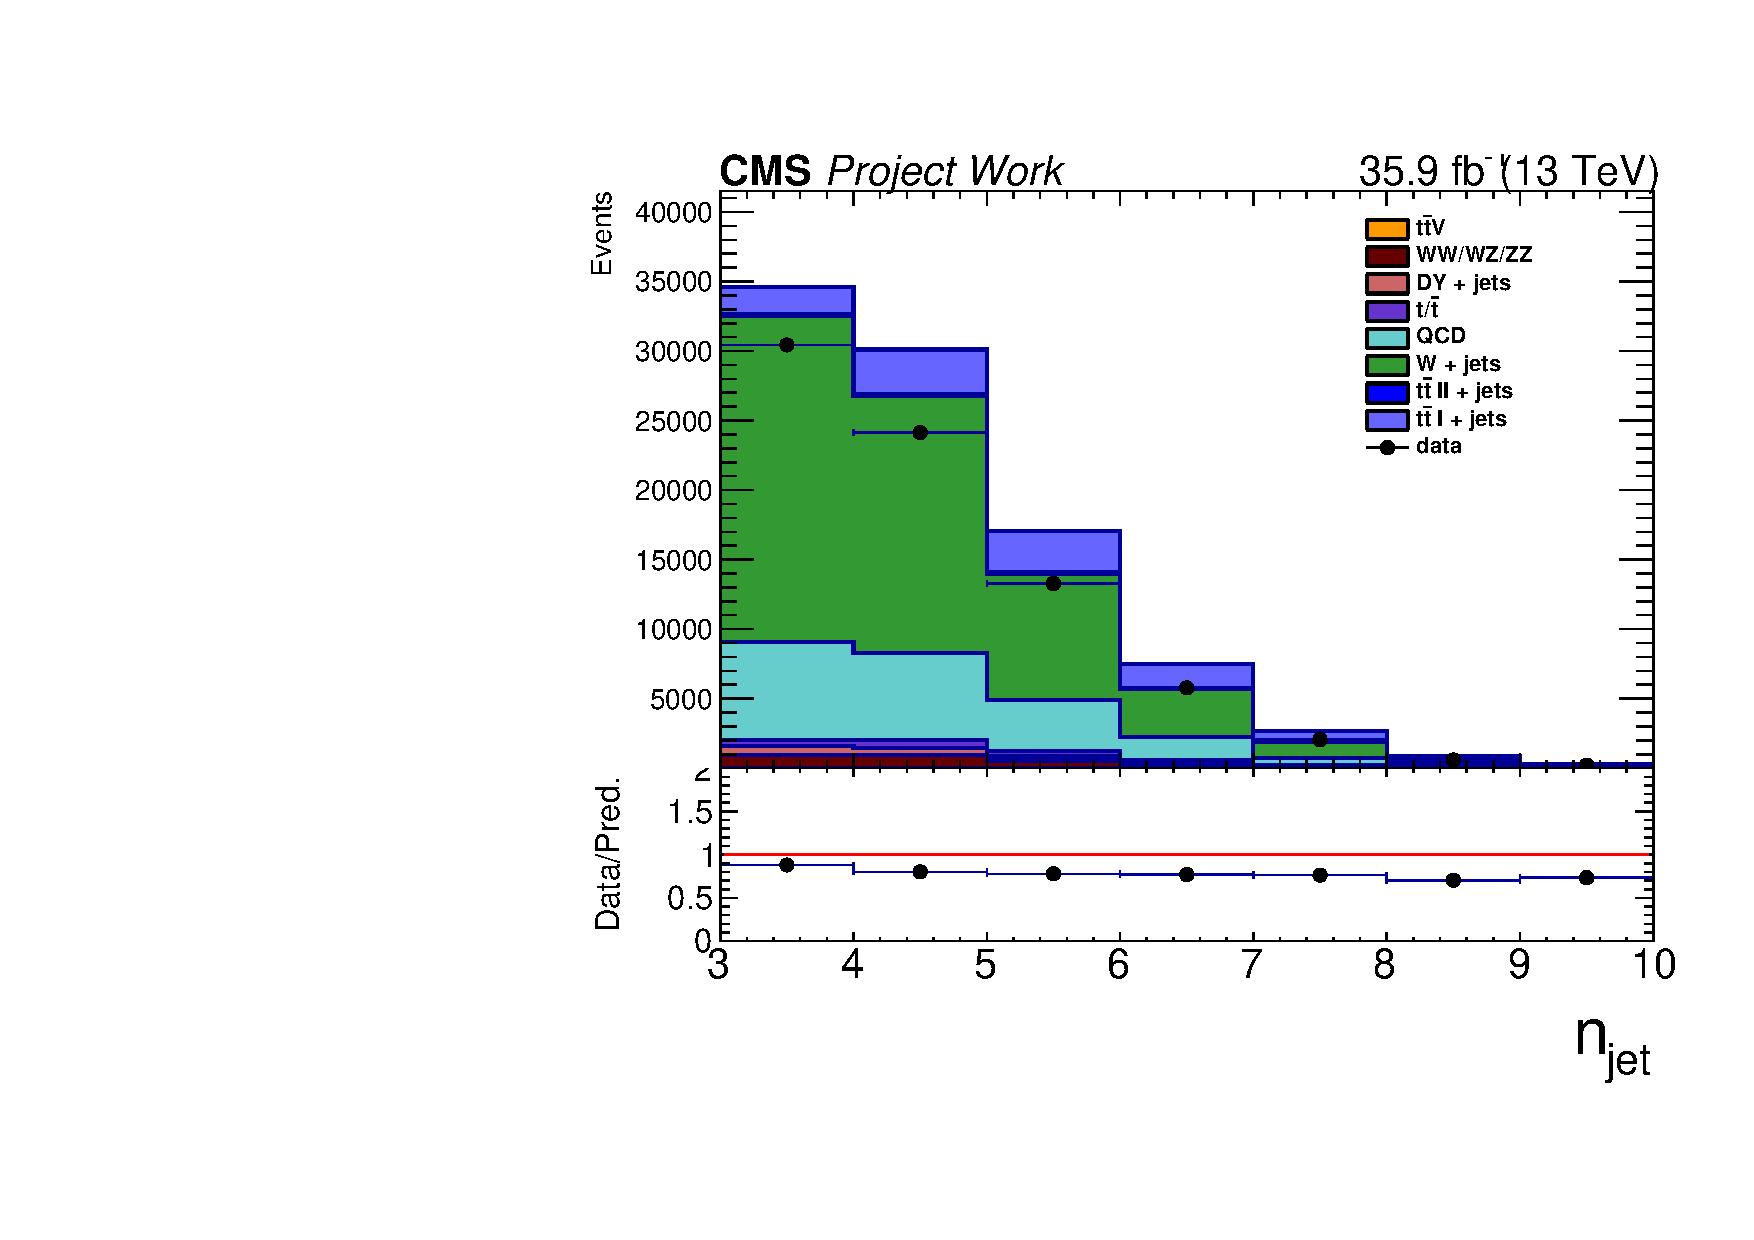
\includegraphics[width=0.45 \textwidth]{PhD_Thesis_v4/Plots/analysis/RCS/diLepCR/nJetSingleFin.pdf}
 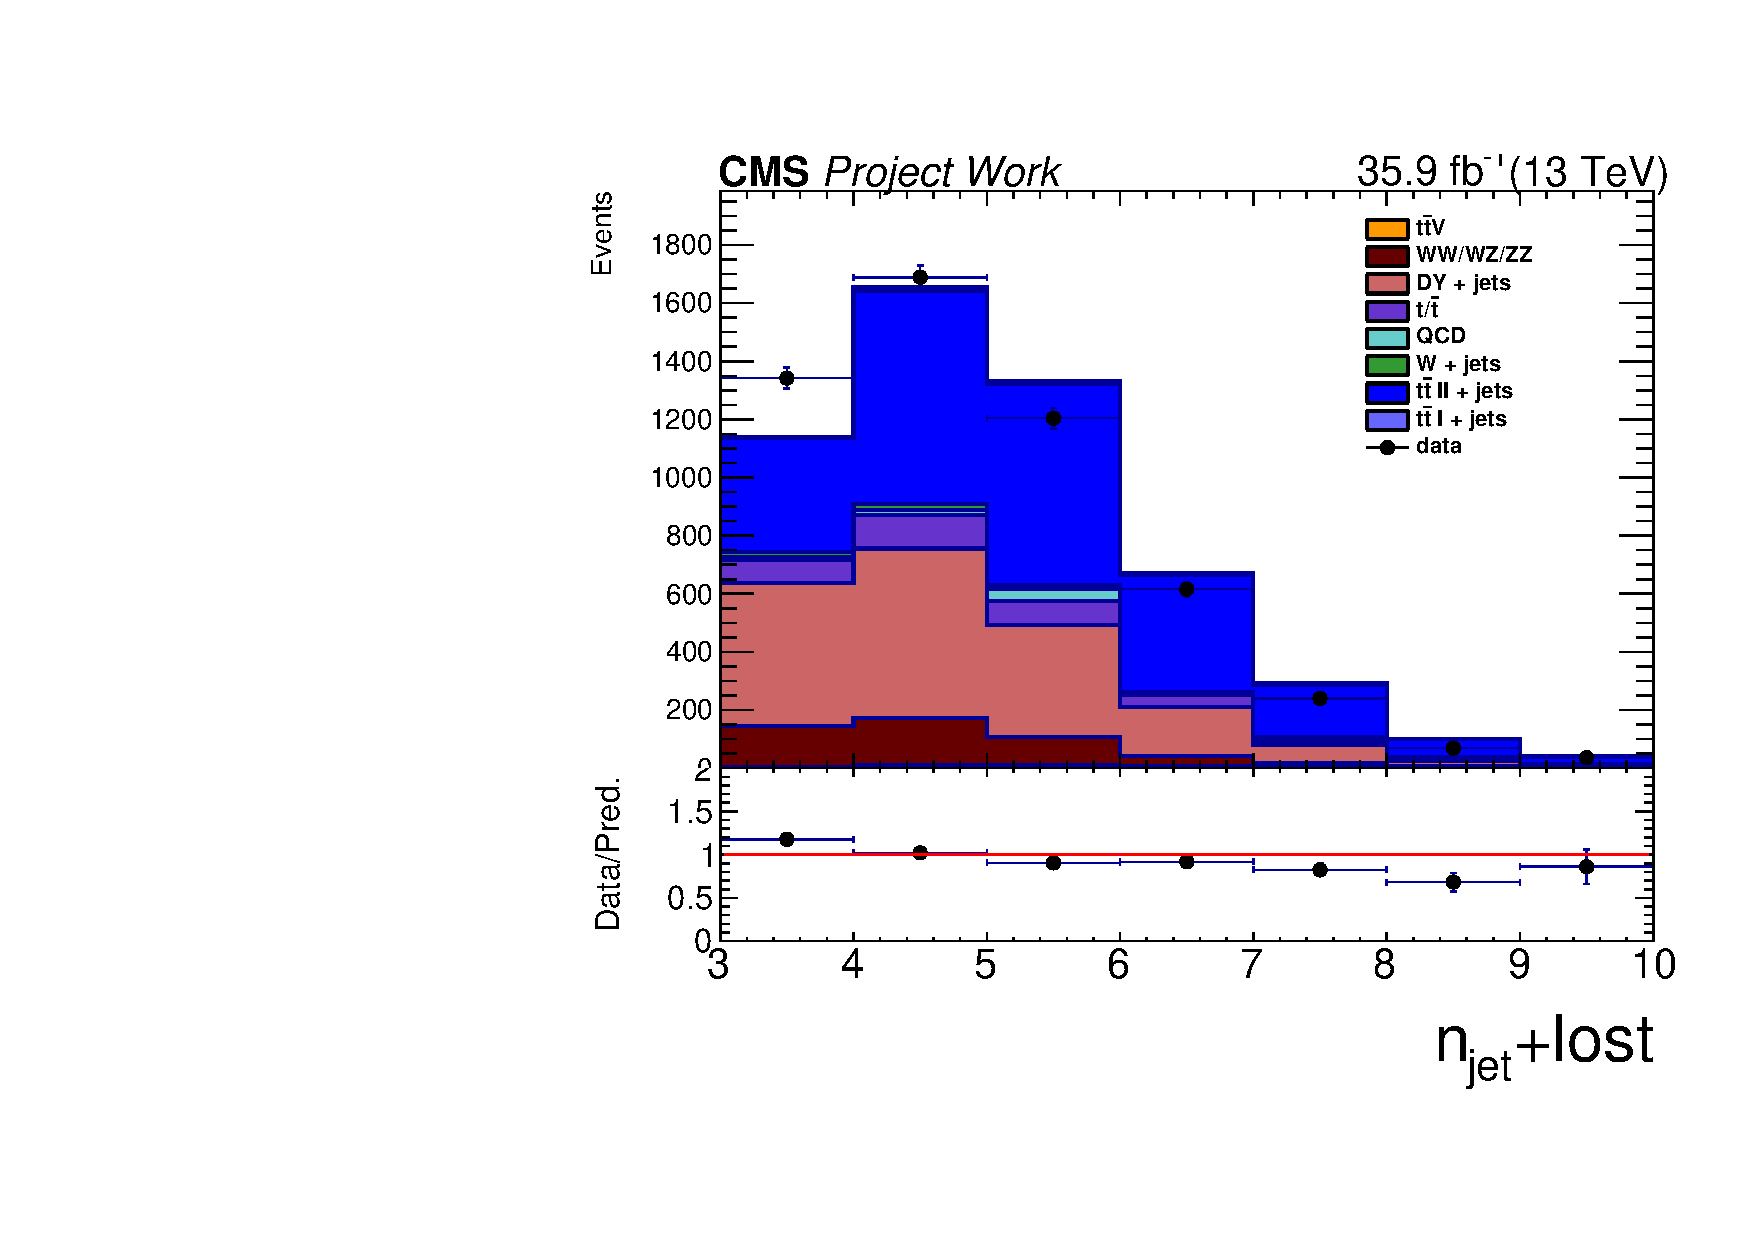
\includegraphics[width=0.45 \textwidth]{PhD_Thesis_v4/Plots/analysis/RCS/diLepCR/nJetdilepFin.pdf}\\
    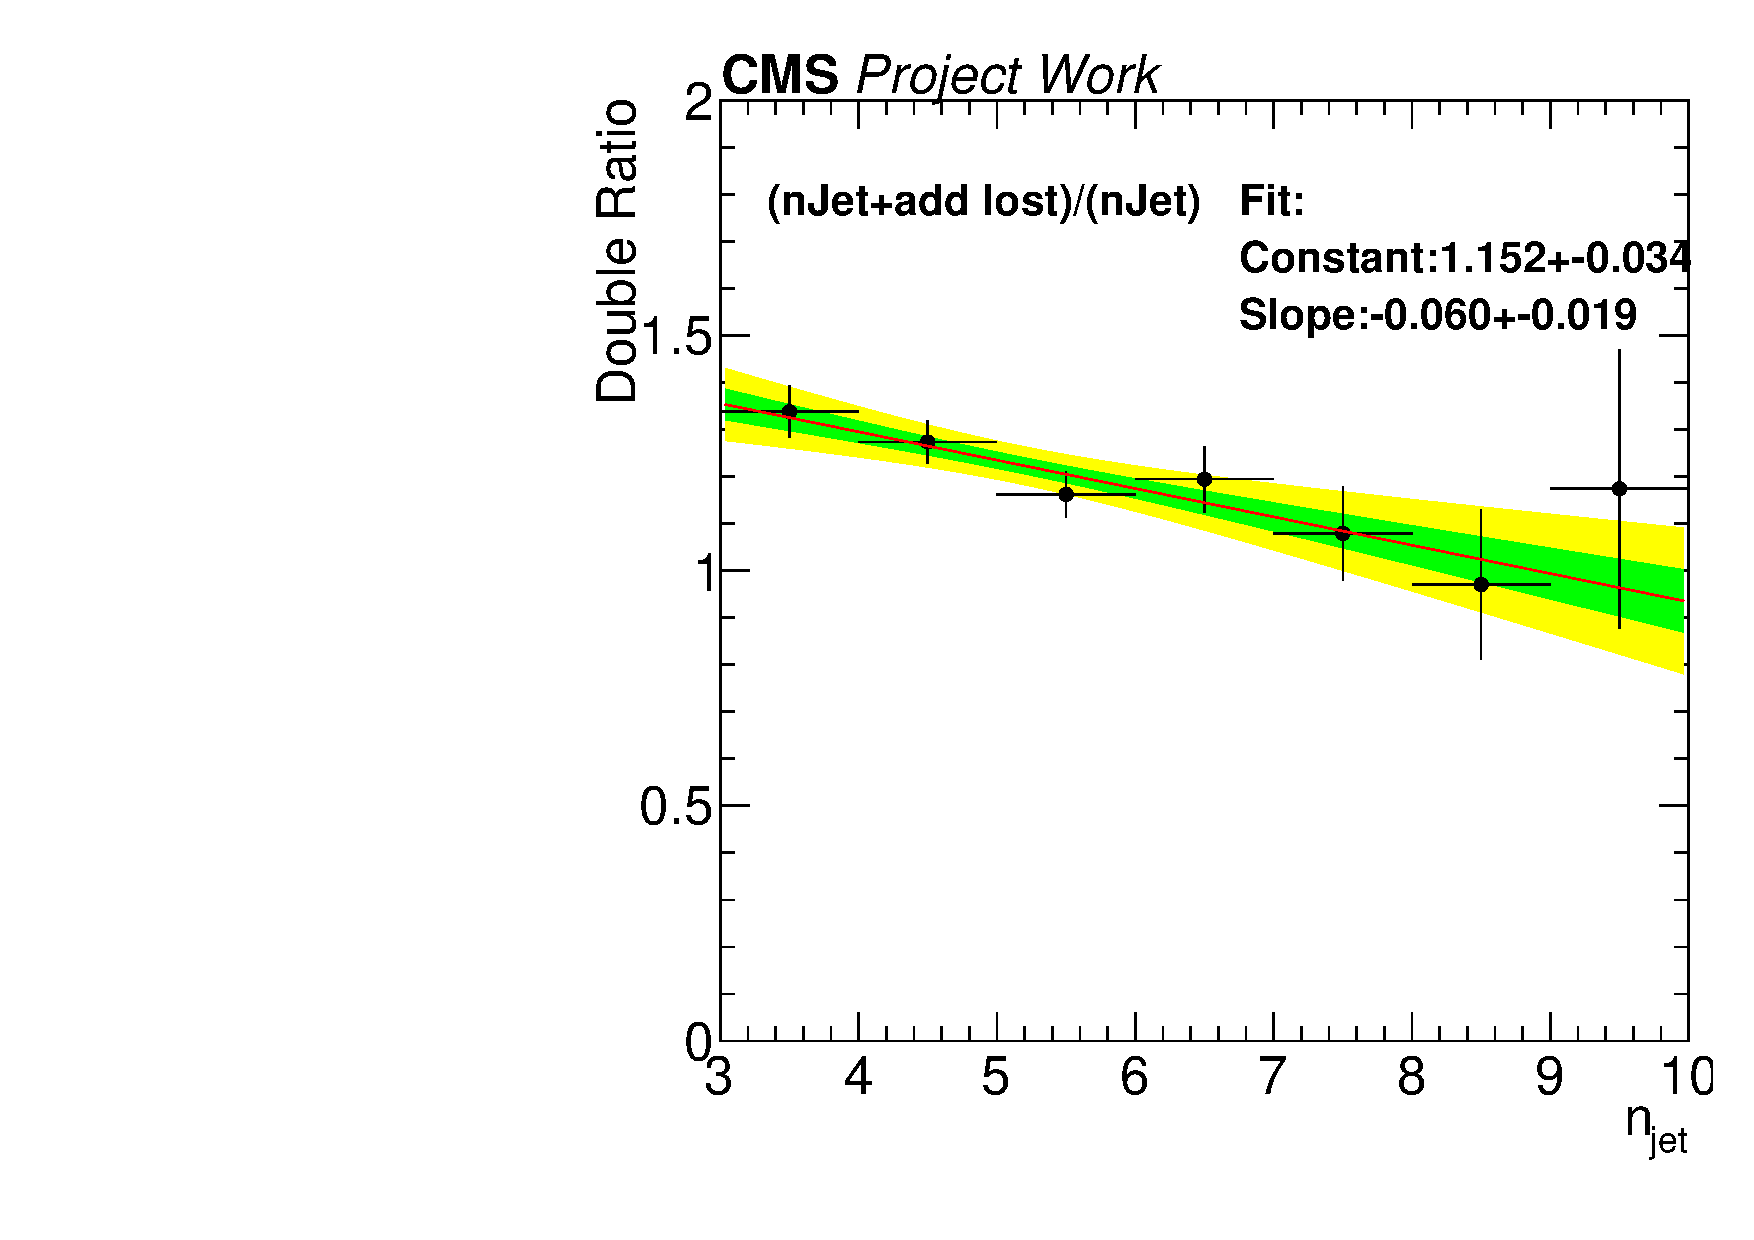
\includegraphics[width=0.4 \textwidth]{PhD_Thesis_v4/Plots/analysis/RCS/diLepCR/nJET_doubleratio.pdf}
  \caption[Double Ratio of $\njet$ distributions]{ \label{dl-CR} Jet multiplicity distribution after the single lepton baseline event selection (in the control region)
 with $\HT>500$ GeV, $\LT>250$ GeV, and $\nbtag = 0$ (left) and in the dileptonic control region with recalculated $\HT$ and $\LT$ cuts (right). Only nISR reweighting is applied. The bottom figure shows the ratio of the distributions in the lower panels of single leptonic~(top left) and dileptonic~(top right) events.}
  \end{center}
\end{figure*}
\newpage
If the simulation described the dileptonic contribution perfectly, this double ratio would be flat at unity. However, it is seen in Fig.~\ref{dl-CR}~(bottom), that the dileptonic events in simulation should be corrected to obtain a $\kappa_{\ttbar}^{DL-corr}$. 
The double ratio in Fig.~\ref{dl-CR}~(bottom) is fitted with a linear parametrization:
\begin{equation}
f(\njet) = a+b(\njet-\langle \njet \rangle), 
\end{equation}
where $\langle \njet \rangle$ is the weighted mean value of $\njet$ in single lepton selection, $a$ determines the offset and $b$ determines the slope.
The weight that is used to rescale dileptonic events are then written as:
\begin{equation}
\label{weight_DL}
{\rm w_{DL}} = {\rm constant}+{\rm slope}\cdot(\njet - \langle \njet \rangle),
\end{equation}
where the $\langle \njet \rangle$ is found to be 5.9, constant and slope values are measured 1.152 and -0.060, respectively.
A new $\kappa_{\ttbar}$, which is denoted by $\kappa_{\ttbar}^{DL-Corr}$, measured as in
Eq.~\ref{eq:kappatt} but this time using the samples in which dileptonic $\ttJets$ events are weighted with $\rm w_{DL}$.
The comparison of $\kappa_{\ttbar}$ before and after correction can be seen in Fig.\ref{fig:kappa_tt}.\\
\begin{figure*}[!htb]
    \begin{center}
 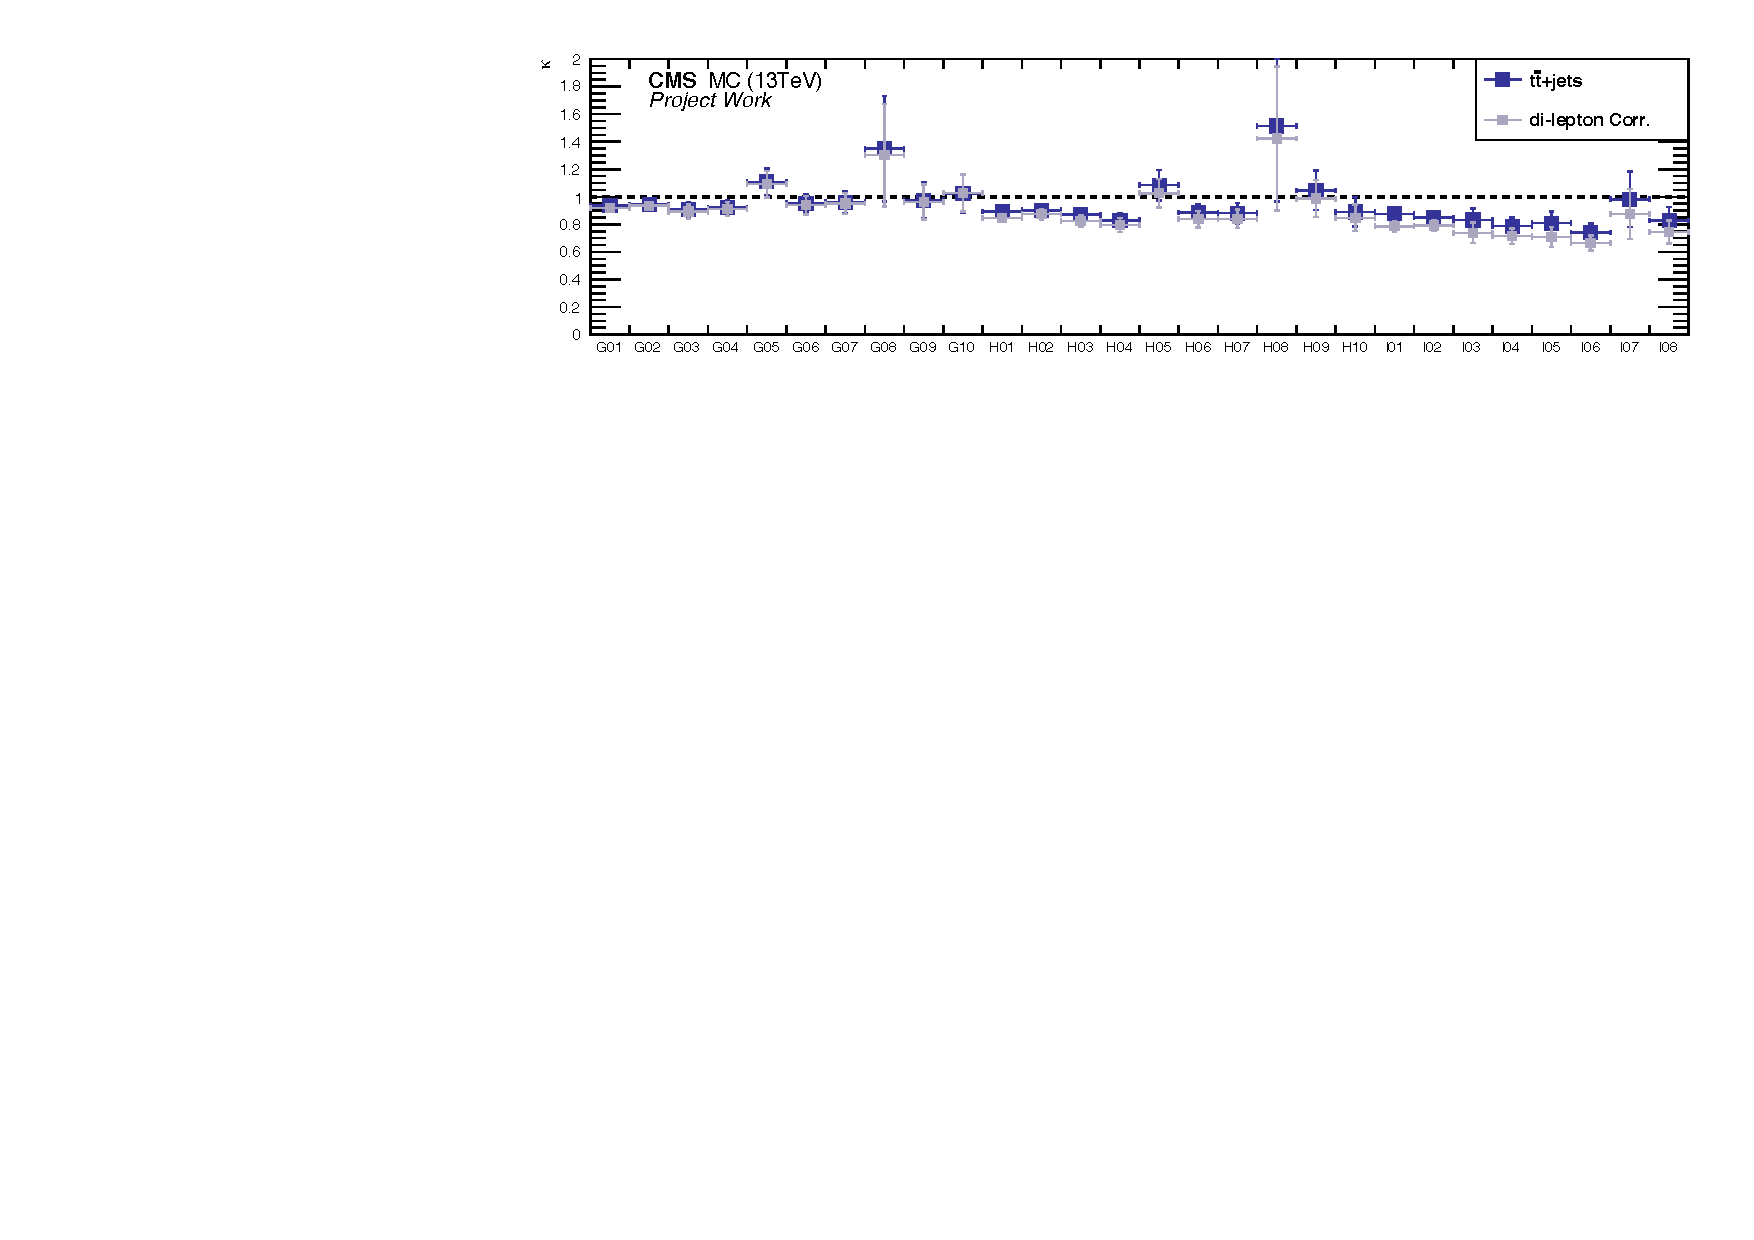
\includegraphics[width=1. \textwidth]{PhD_Thesis_v4/Plots/analysis/RCS/diLepCR/Spring16_templates_SR_Moriond2017_Summer16_lep_MC_SF_Kappa_compForthesis2.pdf}
  \caption[Comparing $\kappa_{\ttbar}$ and $\kappa_{\ttbar}^{DL-Corr}$]{ \label{fig:kappa_tt} Comparing $\kappa_{\ttbar}$ and $\kappa_{\ttbar}^{DL-Corr}$ where the correction accounts for the impact of dileptonic $\ttbar$ events.}
  \end{center}
\end{figure*}
\\
The resulting $\Rcs$ for $\ttJets$ estimation is then written as:
\begin{equation}
\label{Final_RCS}
R^{\ttbar}_{\rm CS}({\rm 0b},{\rm MB}) = {\kappa_b}\cdot{\kappa_{\ttbar}^{DL-Corr}}\cdot{R_{\rm CS}^{data}({\rm b} \geq 1, \njet \in [4,5] )}.
\end{equation}
A summary of $\kappa_b$ corrected $\Rcs$, $\Rcs$ in MB regions from simulation, and different $\kappa$ values are shown in Tab.~\ref{tab:0b_rcs_tt}.
\begin{table}[ht]\begin{center}
\caption{Summary table for $\Rcs$ for $t\bar{t}$+jets and the corresponding $\kappa_{t\bar{t}}$ value from simulation}\label{tab:0b_rcs_tt}
\resizebox{\textwidth}{!}{\begin{tabular}{|c|c|c|rrr|rrr|rrr|rrr|}\hline
 \njet     & \LT & \HT & \multicolumn{3}{c|}{\multirow{2}{*}{$R_{CS}(\textrm{4-5j, b\geq1})\cdot\kappa_{b}^{MC}$}} & \multicolumn{3}{c|}{\multirow{2}{*}{$R_{CS}(\textrm{SR, 0b})$}} & \multicolumn{3}{c|}{$\kappa_{t\bar{t}}$} & \multicolumn{3}{c|}{$\kappa_{b}^{MC}$}\\%\hline
 & $[$GeV$]$ & $[$GeV$]$ & & & & & & & \multicolumn{3}{c|}{SR/SB} & \multicolumn{3}{c|}{0b/b\geq1} \\\hline
\hline
\multirow{10}{*}{\begin{sideways}$5$\end{sideways}}
&\multirow{2}{*}{$[250,350]$}
&$[500,750]$
 & 0.0393&$\pm$&0.0019 & 0.0305&$\pm$&0.0006& 0.92&$\pm$&0.03& 0.95&$\pm$&0.02\\
&
&$\geq750$
 & 0.0498&$\pm$&0.0034 & 0.0375&$\pm$&0.0009& 0.94&$\pm$&0.03& 0.91&$\pm$&0.02\\
\cline{2-15}
&\multirow{2}{*}{$[350,450]$}
&$[500,750]$
 & 0.0316&$\pm$&0.003 & 0.0222&$\pm$&0.001& 0.91&$\pm$&0.06& 1.04&$\pm$&0.04\\
&
&$\geq750$
 & 0.0295&$\pm$&0.0037 & 0.0245&$\pm$&0.0009& 0.93&$\pm$&0.05& 0.93&$\pm$&0.03\\
\cline{2-15}
&\multirow{3}{*}{$[450,650]$}
&$[500,750]$
 & 0.0389&$\pm$&0.006 & 0.0354&$\pm$&0.0024& 1.09&$\pm$&0.1& 1.08&$\pm$&0.06\\
&
&$[750,1250]$
 & 0.0352&$\pm$&0.0057 & 0.0286&$\pm$&0.0014& 0.95&$\pm$&0.07& 1.09&$\pm$&0.05\\
&
&$\geq1250$
 & 0.0354&$\pm$&0.0123 & 0.0396&$\pm$&0.0014& 0.97&$\pm$&0.08& 0.88&$\pm$&0.05\\
\cline{2-15}
&\multirow{3}{*}{$\geq650$}
&$[500,750]$
 & 0.3336&$\pm$&0.1809 & 0.2974&$\pm$&0.0656& 1.31&$\pm$&0.39& 1.7&$\pm$&0.3\\
&
&$[750,1250]$
 & 0.0589&$\pm$&0.0168 & 0.0386&$\pm$&0.0032& 0.94&$\pm$&0.12& 1.24&$\pm$&0.11\\
&
&$\geq1250$
 & 0.0867&$\pm$&0.035 & 0.0505&$\pm$&0.0042& 1.05&$\pm$&0.14& 1.35&$\pm$&0.12\\
\cline{2-15}
\hline
\hline
\multirow{10}{*}{\begin{sideways}$[6,7]$\end{sideways}}
&\multirow{2}{*}{$[250,350]$}
&$[500,1000]$
 & 0.04&$\pm$&0.0017 & 0.0301&$\pm$&0.0005& 0.85&$\pm$&0.02& 0.95&$\pm$&0.02\\
&
&$\geq1000$
 & 0.0652&$\pm$&0.0069 & 0.0408&$\pm$&0.0008& 0.87&$\pm$&0.04& 0.86&$\pm$&0.03\\
\cline{2-15}
&\multirow{2}{*}{$[350,450]$}
&$[500,1000]$
 & 0.0297&$\pm$&0.0025 & 0.021&$\pm$&0.0008& 0.82&$\pm$&0.04& 1.02&$\pm$&0.03\\
&
&$\geq1000$
 & 0.0408&$\pm$&0.0075 & 0.0255&$\pm$&0.0008& 0.8&$\pm$&0.05& 0.89&$\pm$&0.04\\
\cline{2-15}
&\multirow{3}{*}{$[450,650]$}
&$[500,750]$
 & 0.0389&$\pm$&0.006 & 0.0348&$\pm$&0.0029& 1.03&$\pm$&0.11& 1.08&$\pm$&0.06\\
&
&$[750,1250]$
 & 0.0352&$\pm$&0.0057 & 0.0266&$\pm$&0.0013& 0.85&$\pm$&0.06& 1.09&$\pm$&0.05\\
&
&$\geq1250$
 & 0.0354&$\pm$&0.0123 & 0.0363&$\pm$&0.0012& 0.85&$\pm$&0.07& 0.88&$\pm$&0.05\\
\cline{2-15}
&\multirow{3}{*}{$\geq650$}
&$[500,750]$
 & 0.3336&$\pm$&0.1809 & 0.2827&$\pm$&0.0951& 1.21&$\pm$&0.48& 1.7&$\pm$&0.3\\
&
&$[750,1250]$
 & 0.0589&$\pm$&0.0168 & 0.0422&$\pm$&0.0044& 0.98&$\pm$&0.14& 1.24&$\pm$&0.11\\
&
&$\geq1250$
 & 0.0867&$\pm$&0.035 & 0.0413&$\pm$&0.002& 0.82&$\pm$&0.09& 1.35&$\pm$&0.12\\
\cline{2-15}
\hline
\hline
\multirow{8}{*}{\begin{sideways}$\geq8$\end{sideways}}
&\multirow{2}{*}{$[250,350]$}
&$[500,1000]$
 & 0.04&$\pm$&0.0017 & 0.0288&$\pm$&0.0014& 0.77&$\pm$&0.04& 0.95&$\pm$&0.02\\
&
&$\geq1000$
 & 0.0652&$\pm$&0.0069 & 0.0388&$\pm$&0.0012& 0.8&$\pm$&0.04& 0.86&$\pm$&0.03\\
\cline{2-15}
&\multirow{2}{*}{$[350,450]$}
&$[500,1000]$
 & 0.0297&$\pm$&0.0025 & 0.02&$\pm$&0.0019& 0.74&$\pm$&0.08& 1.02&$\pm$&0.03\\
&
&$\geq1000$
 & 0.0408&$\pm$&0.0075 & 0.0243&$\pm$&0.0014& 0.72&$\pm$&0.06& 0.89&$\pm$&0.04\\
\cline{2-15}
&\multirow{2}{*}{$[450,650]$}
&$[500,1250]$
 & 0.0372&$\pm$&0.0043 & 0.0245&$\pm$&0.0024& 0.7&$\pm$&0.07& 1.08&$\pm$&0.04\\
&
&$\geq1250$
 & 0.0354&$\pm$&0.0123 & 0.0302&$\pm$&0.0013& 0.67&$\pm$&0.06& 0.88&$\pm$&0.05\\
\cline{2-15}
&\multirow{2}{*}{$\geq650$}
&$[500,1250]$
 & 0.081&$\pm$&0.0203 & 0.0599&$\pm$&0.0112& 0.89&$\pm$&0.19& 1.33&$\pm$&0.11\\
&
&$\geq1250$
 & 0.0867&$\pm$&0.035 & 0.0395&$\pm$&0.0019& 0.74&$\pm$&0.09& 1.35&$\pm$&0.12\\
\cline{2-15}
\hline\end{tabular}}\end{center}\end{table}
\section{$R_{CS}$ method in $\wJets$ events}
\label{sec:RcsW}
For the $\wJets$ estimation, we first note that we need not separately estimate WV(V$=$~W, Z) if the boson V decays hadronically. The contribution from leptonic V decays is a subleading uncertainty in the main analysis and taken from simulation in the SBs.
%In the $\wJets$ background estimation, the $WV$ diboson events, where V stands for $W or Z$ bosons, are included in the prediction mechanism. In the diboson events, which are considered as a part of $\wJets$ estimation, the W boson decays leptonically and the second boson, denoted by V, decays hadronically. The similarity of the kinematics of the events, hence the $\Rcs$ values, makes this addition possible. All other diboson events are treated as part of the rare EWK backgrounds and taken from simulation.\\
For the main measurement of $\Rcs$ values for $\wJets$ background estimation, we define a sideband region with three or four jets. To suppress the $\ttJets$ events and to be kinematically as close as possible to mainband regions, we further veto events with b-tagged jets. 
Furthermore, in order to suppress QCD multijet contamination, $\Rcs$ is measured only in the muon channel, where no QCD multijet subtraction scheme is needed. The $\ttJets$ contamination in the $\wJets$ SB is subtracted from SRs and CRs. Its fraction $f_{\ttbar}$ in the SB~CR is taken again from a b tag multiplicity fit, and $\Rcs^{\ttbar, {\rm MC}}$, that is used to obtain the $\ttJets$ contamination in the $\wJets$ SB~SR, can be taken from simulation.
The $\Rcs$ can then be written as:
\begin{equation}
\label{RCSw}
{\Rcs^{\rm corr. data}({\rm 0b},\njet \in [3,4])} = \frac{N^{SR}_{data}-\Rcs^{\ttbar, {\rm MC}}\cdot f^{fit}_{\ttbar}\cdot N^{CR}_{data}}{(1-f^{fit}_{\ttbar})\cdot N^{CR}_{data}}.
\end{equation}
As already discussed in Sec.~\ref{sec:bkgcomp}, $\Rcs$ is separately measured for positive and negative charged leptons to account for the charged asymmetry of the $\wJets$ events. The simulated $\Rcs^{\rm MC}$ values and the corrected measured $\Rcs$ in events with 3 and 4 jets, with the b~jet veto applied, are given in Tab.~\ref{tab:rcsWsimdata}.\\
\begin{table}[ht]\begin{center}
\caption[The $\Rcs$ values for positively and negatively charged leptons.]{The simulated $\Rcs$ values and the corrected measured $\Rcs$ (as in Eq.~\ref{RCSw}) in events with 3 and 4 jets, 0 b-tagged jet are shown separately for positively and negatively charged leptons.}\label{tab:rcsWsimdata}
\resizebox{\textwidth}{!}{\begin{tabular}{c|c|c|rrr|rrr|rrr|rrr|}\hline
 \multirow{2}{*}{\njet}     &  \multirow{2}{*}{\LT}      &  \multirow{2}{*}{\HT}     & \multicolumn{12}{c|}{$\Rcs$ in 3-4j, 0b}\\%\hline
                             &           &         &\multicolumn{6}{c|}{$\ell^{+}$} &\multicolumn{6}{c|}{$\ell^{-}$}         \\\cline{4-15}
                             & $[$GeV$]$ &$[$GeV$]$& \multicolumn{3}{c|}{simulated} &\multicolumn{3}{c|}{measured}&\multicolumn{3}{c|}{simulated} &\multicolumn{3}{c|}{measured} \\\hline
\hline
\multirow{10}{*}{\begin{sideways}$5$\end{sideways}}
&\multirow{2}{*}{$[250,350]$}
&$[500,750]$
 & 0.0098&$\pm$&0.0005& 0.0142&$\pm$&0.0023& 0.0155&$\pm$&0.0005& 0.0242&$\pm$&0.0021
 \\
&
&$\geq750$
 & 0.0219&$\pm$&0.0009& 0.0347&$\pm$&0.0057& 0.0275&$\pm$&0.0008& 0.0403&$\pm$&0.0045
 \\
\cline{2-15}
&\multirow{2}{*}{$[350,450]$}
&$[500,750]$
 & 0.0044&$\pm$&0.0005& 0.0094&$\pm$&0.0029& 0.0067&$\pm$&0.0005& 0.0116&$\pm$&0.0022
 \\
&
&$\geq750$
 & 0.01&$\pm$&0.0009& 0.0169&$\pm$&0.0059& 0.0129&$\pm$&0.0008& 0.0252&$\pm$&0.005
 \\
\cline{2-15}
&\multirow{3}{*}{$[450,650]$}
&$[500,750]$
 & 0.0076&$\pm$&0.0008& 0.0105&$\pm$&0.0036& 0.0102&$\pm$&0.0007& 0.0136&$\pm$&0.0029
 \\
&
&$[750,1250]$
 & 0.0078&$\pm$&0.0009& 0.0189&$\pm$&0.0068& 0.0106&$\pm$&0.0007& 0.0125&$\pm$&0.004
 \\
&
&$\geq1250$
 & 0.0206&$\pm$&0.0043& 0.0059&$\pm$&0.0168& 0.0213&$\pm$&0.0034& 0.0612&$\pm$&0.0257
 \\
\cline{2-15}
&\multirow{3}{*}{$\geq650$}
&$[500,750]$
 & 0.0468&$\pm$&0.007& 0.0143&$\pm$&0.0144& 0.0472&$\pm$&0.0051& 0.1287&$\pm$&0.0379
 \\
&
&$[750,1250]$
 & 0.0104&$\pm$&0.0013& 0.0133&$\pm$&0.0088& 0.0211&$\pm$&0.0013& 0.0326&$\pm$&0.0092
 \\
&
&$\geq1250$
 & 0.0185&$\pm$&0.0048& 0.0349&$\pm$&0.0289& 0.0207&$\pm$&0.0035& 0.0339&$\pm$&0.0172
 \\
\cline{2-15}
\hline
\hline
\multirow{10}{*}{\begin{sideways}$[6,7]$\end{sideways}}
&\multirow{2}{*}{$[250,350]$}
&$[500,1000]$
 & 0.0112&$\pm$&0.0004& 0.0178&$\pm$&0.0023& 0.0169&$\pm$&0.0004& 0.027&$\pm$&0.002
 \\
&
&$\geq1000$
 & 0.033&$\pm$&0.0023& 0.0381&$\pm$&0.0107& 0.0371&$\pm$&0.0019& 0.0439&$\pm$&0.0082
 \\
\cline{2-15}
&\multirow{2}{*}{$[350,450]$}
&$[500,1000]$
 & 0.005&$\pm$&0.0004& 0.0107&$\pm$&0.0027& 0.0073&$\pm$&0.0004& 0.0132&$\pm$&0.002
 \\
&
&$\geq1000$
 & 0.0157&$\pm$&0.0023& 0.0191&$\pm$&0.0102& 0.0187&$\pm$&0.0019& 0.0377&$\pm$&0.0106
 \\
\cline{2-15}
&\multirow{3}{*}{$[450,650]$}
&$[500,750]$
 & 0.0076&$\pm$&0.0008& 0.0105&$\pm$&0.0036& 0.0102&$\pm$&0.0007& 0.0136&$\pm$&0.0029
 \\
&
&$[750,1250]$
 & 0.0078&$\pm$&0.0009& 0.0189&$\pm$&0.0068& 0.0106&$\pm$&0.0007& 0.0125&$\pm$&0.004
 \\
&
&$\geq1250$
 & 0.0206&$\pm$&0.0043& 0.0059&$\pm$&0.0168& 0.0213&$\pm$&0.0034& 0.0612&$\pm$&0.0257
 \\
\cline{2-15}
&\multirow{3}{*}{$\geq650$}
&$[500,750]$
 & 0.0468&$\pm$&0.007& 0.0143&$\pm$&0.0144& 0.0472&$\pm$&0.0051& 0.1287&$\pm$&0.0379
 \\
&
&$[750,1250]$
 & 0.0104&$\pm$&0.0013& 0.0133&$\pm$&0.0088& 0.0211&$\pm$&0.0013& 0.0326&$\pm$&0.0092
 \\
&
&$\geq1250$
 & 0.0185&$\pm$&0.0048& 0.0349&$\pm$&0.0289& 0.0207&$\pm$&0.0035& 0.0339&$\pm$&0.0172
 \\
\cline{2-15}
\hline
\hline
\multirow{8}{*}{\begin{sideways}$\geq8$\end{sideways}}
&\multirow{2}{*}{$[250,350]$}
&$[500,1000]$
 & 0.0112&$\pm$&0.0004& 0.0178&$\pm$&0.0023& 0.0169&$\pm$&0.0004& 0.027&$\pm$&0.002
 \\
&
&$\geq1000$
 & 0.033&$\pm$&0.0023& 0.0381&$\pm$&0.0107& 0.0371&$\pm$&0.0019& 0.0439&$\pm$&0.0082
 \\
\cline{2-15}
&\multirow{2}{*}{$[350,450]$}
&$[500,1000]$
 & 0.005&$\pm$&0.0004& 0.0107&$\pm$&0.0027& 0.0073&$\pm$&0.0004& 0.0132&$\pm$&0.002
 \\
&
&$\geq1000$
 & 0.0157&$\pm$&0.0023& 0.0191&$\pm$&0.0102& 0.0187&$\pm$&0.0019& 0.0377&$\pm$&0.0106
 \\
\cline{2-15}
&\multirow{2}{*}{$[450,650]$}
&$[500,1250]$
 & 0.0077&$\pm$&0.0006& 0.0132&$\pm$&0.0033& 0.0104&$\pm$&0.0005& 0.0132&$\pm$&0.0024
 \\
&
&$\geq1250$
 & 0.0206&$\pm$&0.0043& 0.0059&$\pm$&0.0168& 0.0213&$\pm$&0.0034& 0.0612&$\pm$&0.0257
 \\
\cline{2-15}
&\multirow{2}{*}{$\geq650$}
&$[500,1250]$
 & 0.018&$\pm$&0.0018& 0.013&$\pm$&0.0075& 0.0267&$\pm$&0.0015& 0.052&$\pm$&0.0105
 \\
&
&$\geq1250$
 & 0.0185&$\pm$&0.0048& 0.0349&$\pm$&0.0289& 0.0207&$\pm$&0.0035& 0.0339&$\pm$&0.0172
 \\
\cline{2-15}
\hline\end{tabular}}\end{center}\end{table}
\begin{figure*}[!hbt]
    \begin{center}
 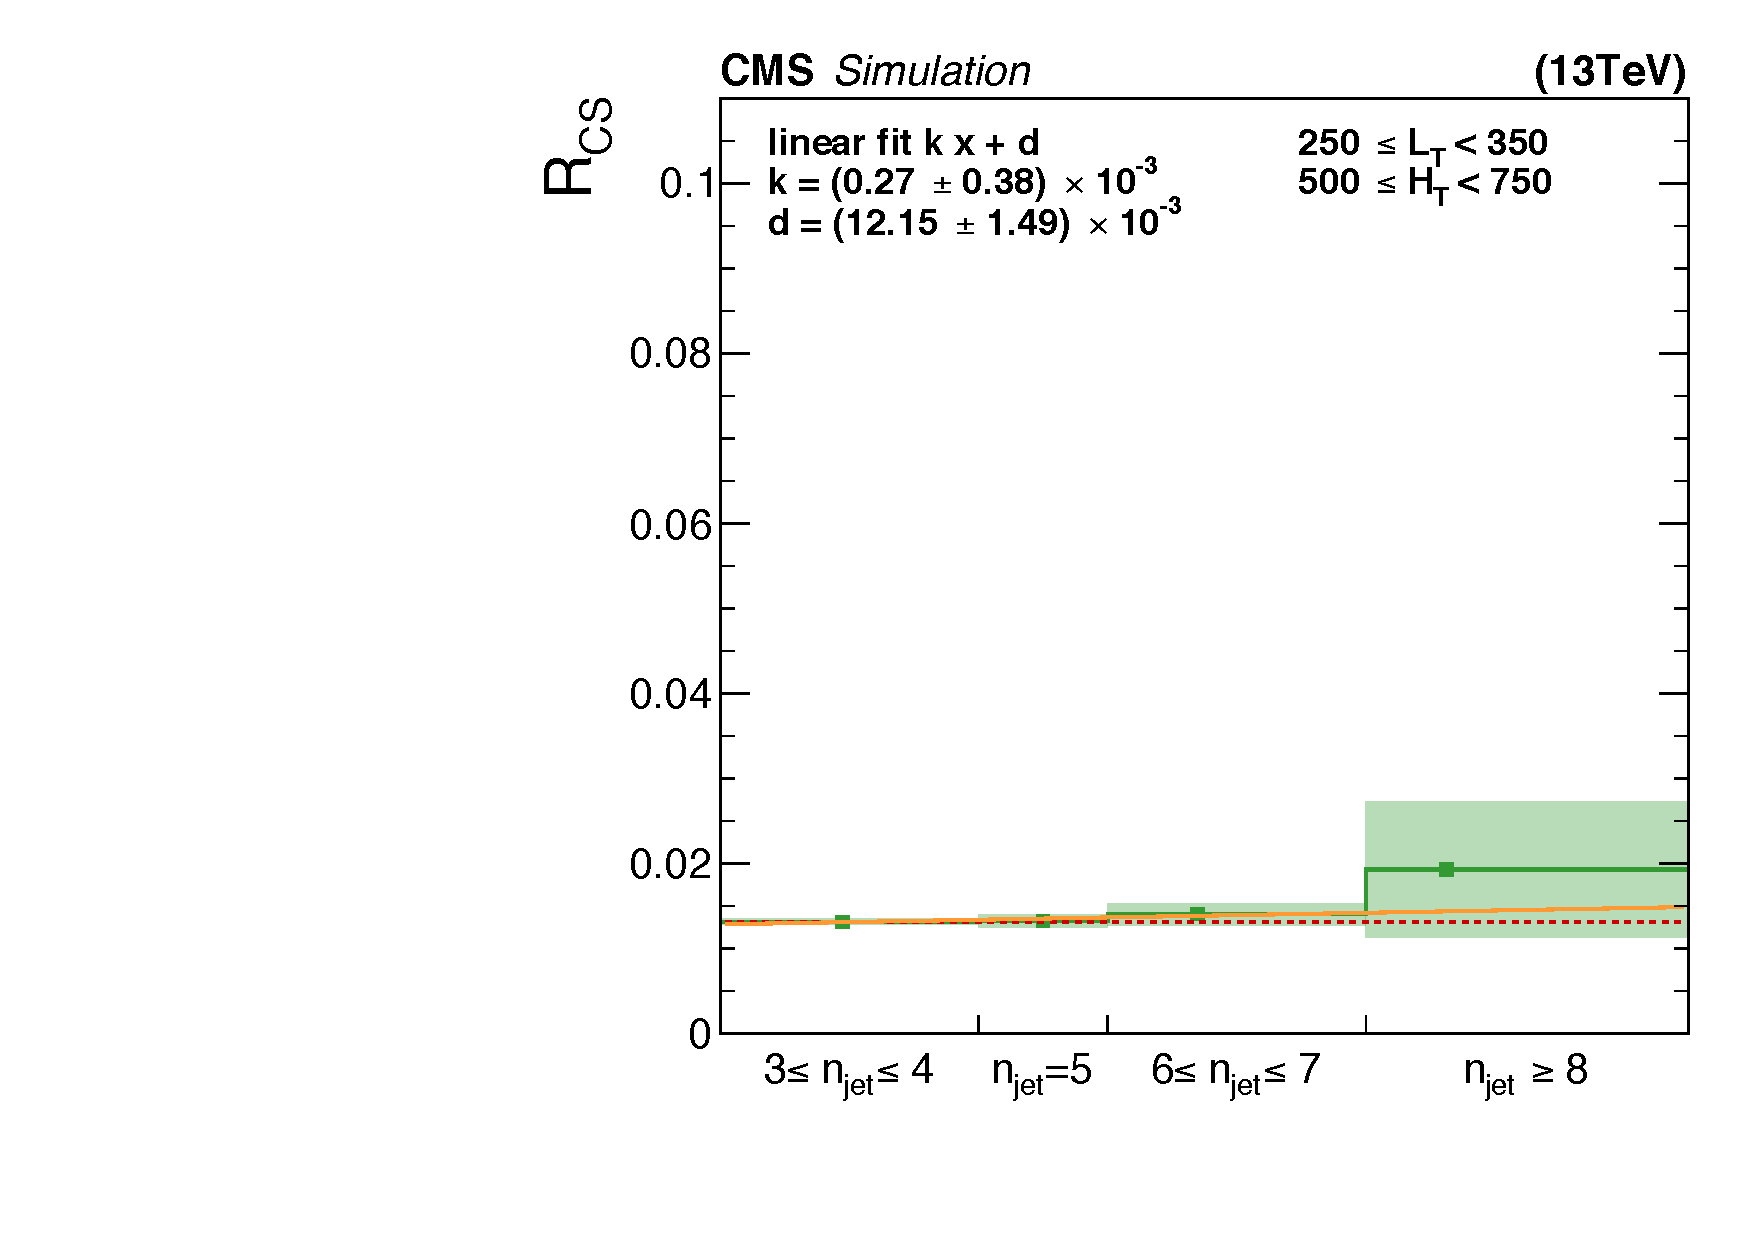
\includegraphics[width=0.45 \textwidth]{PhD_Thesis_v4/Plots/analysis/RCS/st250-350_ht500-750_njet8_nbtag0_Wjets_all_fit.pdf}
   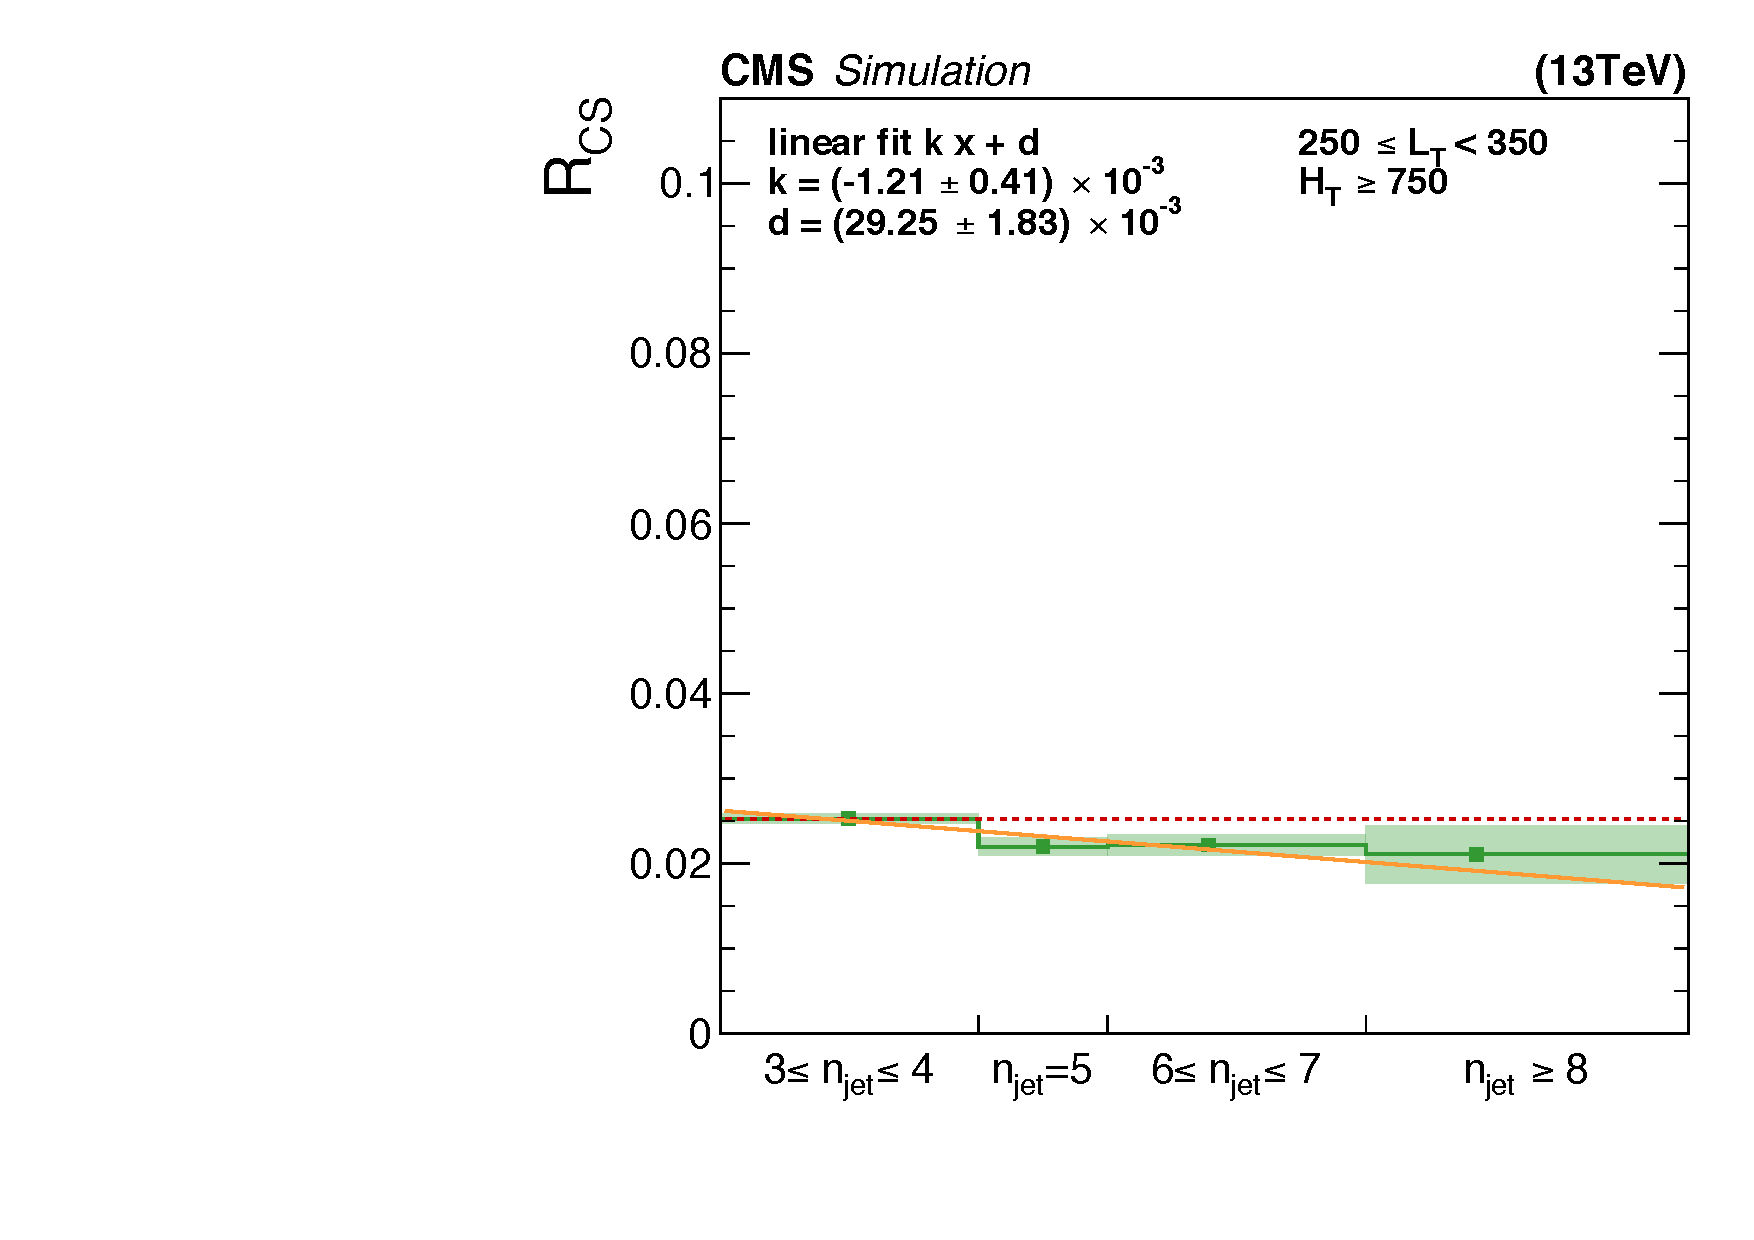
\includegraphics[width=0.45 \textwidth]{PhD_Thesis_v4/Plots/analysis/RCS/st250-350_ht750_njet8_nbtag0_Wjets_all_fit.pdf}
  \caption[Simulated $\Rcs$ for $\wJets$ events]{ \label{RCS_dataMCw} $\Rcs$ as a function of $\njet$ from simulation:  low $\HT$~(left), and high $\HT$~(right) values for the first search bin which is $\njet =$~5, $\LT \in$~[250,350]~GeV.}
  \end{center}
\end{figure*}
Figure~\ref{RCS_dataMCw} shows simulated $\Rcs$ in low $\HT$(left), and high $\HT$ (right) values for the first search bin which is defined by $\njet =$~5, $\LT \in$~[250,350]~GeV.\\
Again, as in the $\ttbar$ case, residual differences between the $\Rcs$ in the sideband and mainband are calculated in simulation as a correction factor $\kappa$. This time, only one $\kappa$ factor is used, due to the fact that the sideband and mainband regions are sharing the same requirement for number of b-tagged jets, $\nbtag=$~0. The factor $\kappa_w$ accounts for residual dependence of $\Rcs$ on the jet multiplicity and also covers variations of $\Rcs$ values in the muon channel and the inclusive single lepton channel. The factor $\kappa_w$ is calculated as:
\begin{equation}
\label{kappa_w}
\kappa_w = \frac{\Rcs^{MC}({\rm 0b},\njet {\rm \,as\,in\,MB},\wJets)}{R^{corr, MC}_{CS}(0b,\njet \in [3,4],\mu)}.
\end{equation}
Resulting in:
\begin{equation}
\Rcs^{W}({\rm 0b},{\rm MB}) = {\kappa_w}\cdot{\Rcs^{\rm corr. data}({\rm 0b},\njet \in [3,4], \mu)}.
\end{equation}
Fig.~\ref{fig:kappaW} shows the $\kappa_w$ values in the lower panel and the $\Rcs$ values went into this calculation in the upper panel. In two kinematically extreme bins of high $\LT$ and low $\HT$ the $\Rcs$ values are different from the bulk but the SB follows the MB, therefore, $\kappa_w$ values are still compatible with 1.
\begin{figure*}[!hbt]
    \begin{center}
 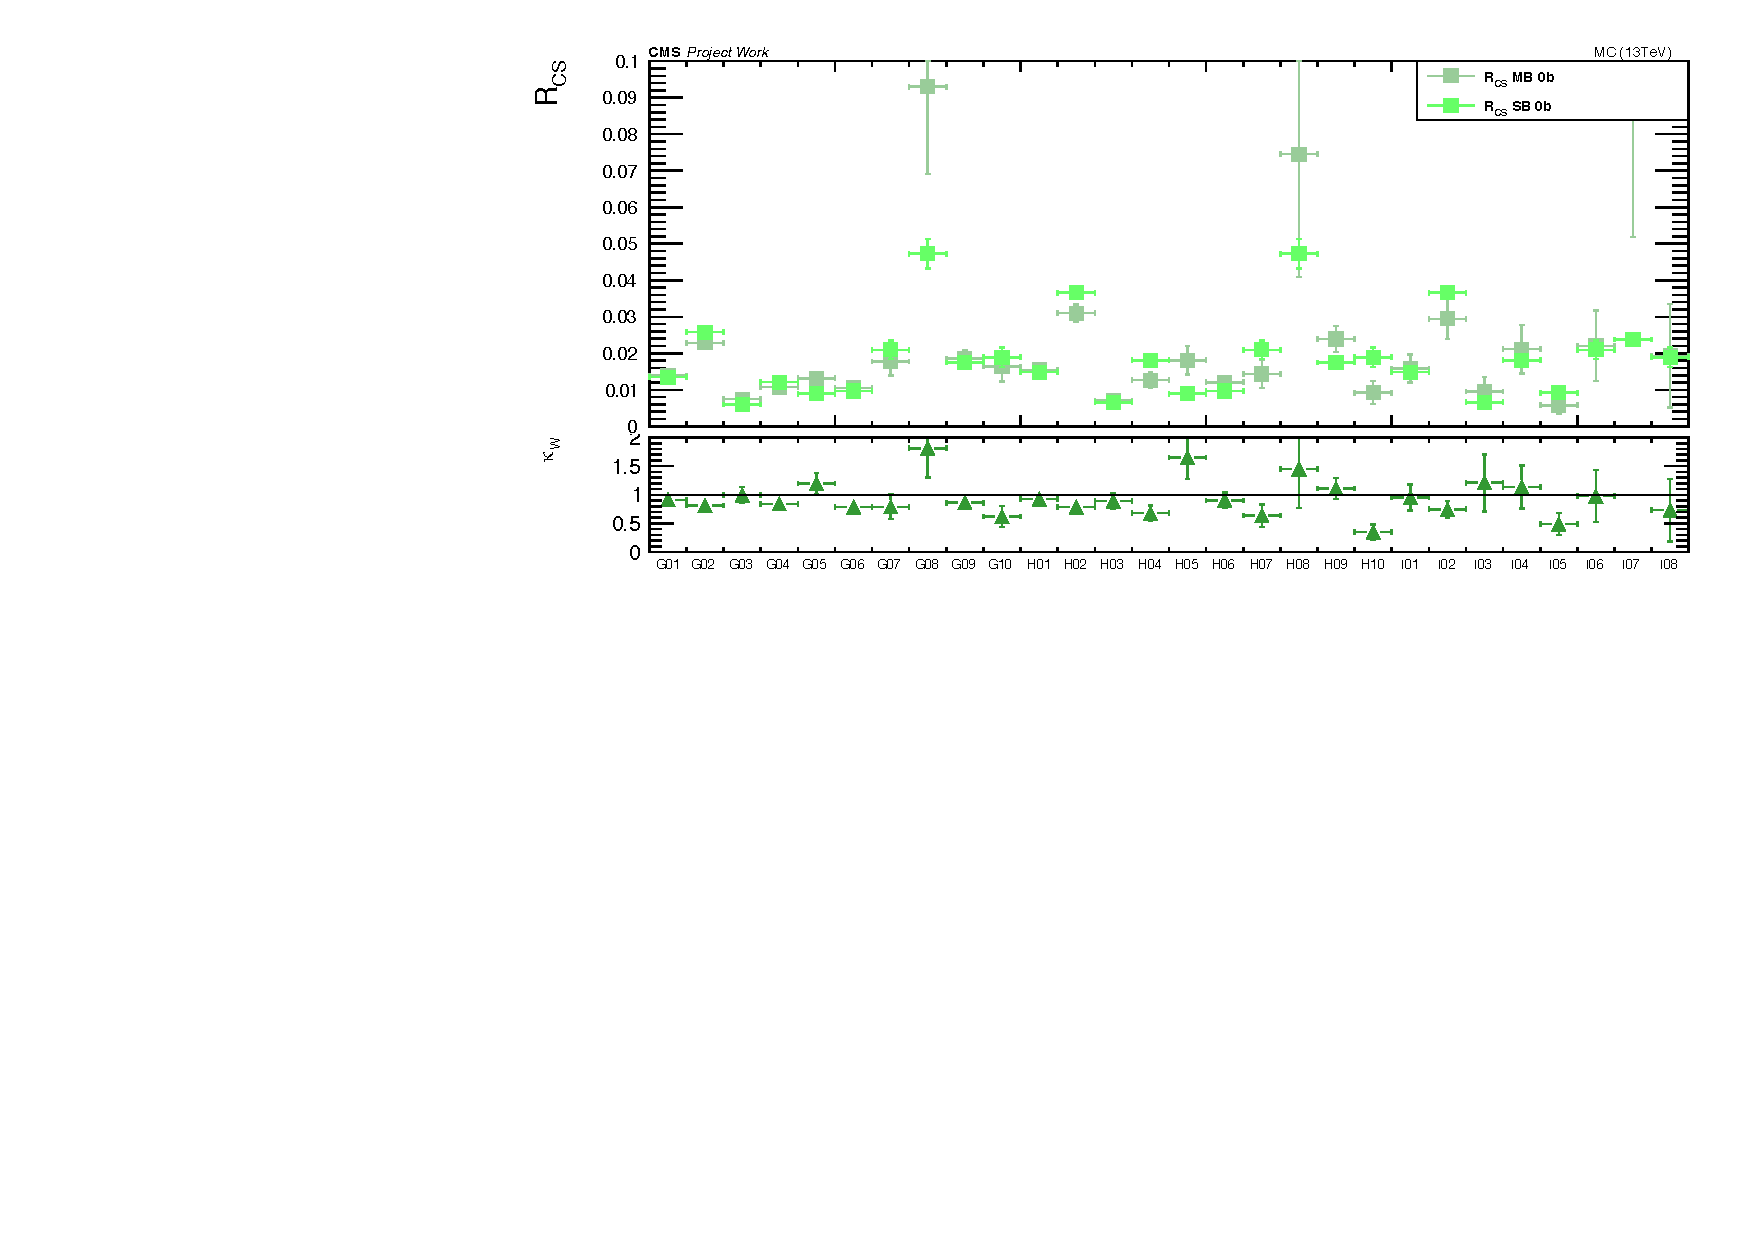
\includegraphics[width=1. \textwidth]{PhD_Thesis_v4/Plots/analysis/RCS/kappaW.pdf}
  \caption{ \label{fig:kappaW} The top row shows the two simulated $\Rcs$ values~(Eq.~\ref{kappa_w} numerator and denominator). The bottom row shows the resulting $\kappa_w$.}
  \end{center}
\end{figure*}
\section{Validation of the background estimation}
\label{sec:Val}
A Validation of the background estimation method is performed in events where there are four jets and zero b-tagged jets.
This region is a part of the $\wJets$ sideband of the main estimation and it is dominated by the SM background events. Consequently, in the validation, to perform the $\wJets$ prediction, only $\njet=$~3 selection is used as the sideband. The $\ttJets$ sideband remains unchanged since, it is not used as the validation search region. The simulated signal and background yields, together with the bin naming, can be found in Tab.~\ref{tab:ValSim}. Fig.~\ref{kappaVal} presents the obtained $\kappa_w^{\rm val}$ and $\kappa_{\ttbar}^{\rm val}$ values.
\begin{table}[ht]\begin{center}
\caption{Simulation table of the validation regions, 35.9~fb$^{-1}$}\label{tab:ValSim}
\resizebox{\textwidth}{!}{\begin{tabular}{c|c|c|l|rrr|rrr|rrr|rrr|}\hline
 \multirow{2}{*}{\njet}     & \LT & \HT     & \multirow{2}{*}{Bin name} & \multicolumn{6}{c|}{T5qqqqWW $m_{gl}$/$m_{\ninozero}$ $[$TeV$]$} & \multicolumn{3}{c|}{tot. background} \\%\hline
 & $[$GeV$]$ &$[$GeV$]$ &   & \multicolumn{3}{c}{(1.5/1.0)} & \multicolumn{3}{c|}{(1.9/0.1)} & \multicolumn{3}{c|}{Simulation}  \\\hline
\hline
\multirow{8}{*}{\begin{sideways}$4$\end{sideways}}
&\multirow{2}{*}{$[250,350]$}
&$[500,1000]$
 & $\textrm{LT0},  \textrm{HT01}$
 & 0.8&$\pm$&0.21 & 0.01&$\pm$&0.01 & 250.18&$\pm$&10.28
 &  \\
&
&$\geq1000$
 & $\textrm{LT0},  \textrm{HT2i}$
 & 0.0&$\pm$&0.0 & 0.01&$\pm$&0.01 & 63.61&$\pm$&3.64
 &  \\
\cline{2-13}
&\multirow{2}{*}{$[350,450]$}
&$[500,1000]$
 & $\textrm{LT1},  \textrm{HT01}$
 & 0.96&$\pm$&0.23 & 0.01&$\pm$&0.01 & 64.88&$\pm$&4.74
 &  \\
&
&$\geq1000$
 & $\textrm{LT1},  \textrm{HT2i}$
 & 0.11&$\pm$&0.08 & 0.0&$\pm$&0.0 & 17.46&$\pm$&1.96
 &  \\
\cline{2-13}
&\multirow{2}{*}{$[450,650]$}
&$[500,1000]$
 & $\textrm{LT2},  \textrm{HT01}$
 & 1.61&$\pm$&0.29 & 0.01&$\pm$&0.01 & 60.66&$\pm$&4.83
 &  \\
&
&$\geq1000$
 & $\textrm{LT2},  \textrm{HT2i}$
 & 0.05&$\pm$&0.05 & 0.07&$\pm$&0.02 & 16.65&$\pm$&1.66
 &  \\
\cline{2-13}
&\multirow{2}{*}{$\geq650$}
&$[500,1000]$
 & $\textrm{LT3i},  \textrm{HT01}$
 & 0.48&$\pm$&0.16 & 0.03&$\pm$&0.01 & 26.46&$\pm$&3.32
 &  \\
&
&$\geq1000$
 & $\textrm{LT3i},  \textrm{HT2i}$
 & 0.0&$\pm$&0.0 & 0.31&$\pm$&0.05 & 13.49&$\pm$&1.5
 &  \\
\cline{2-13}
\hline\end{tabular}}\end{center}\end{table}
\begin{figure*}[!hbt]
    \begin{center}
 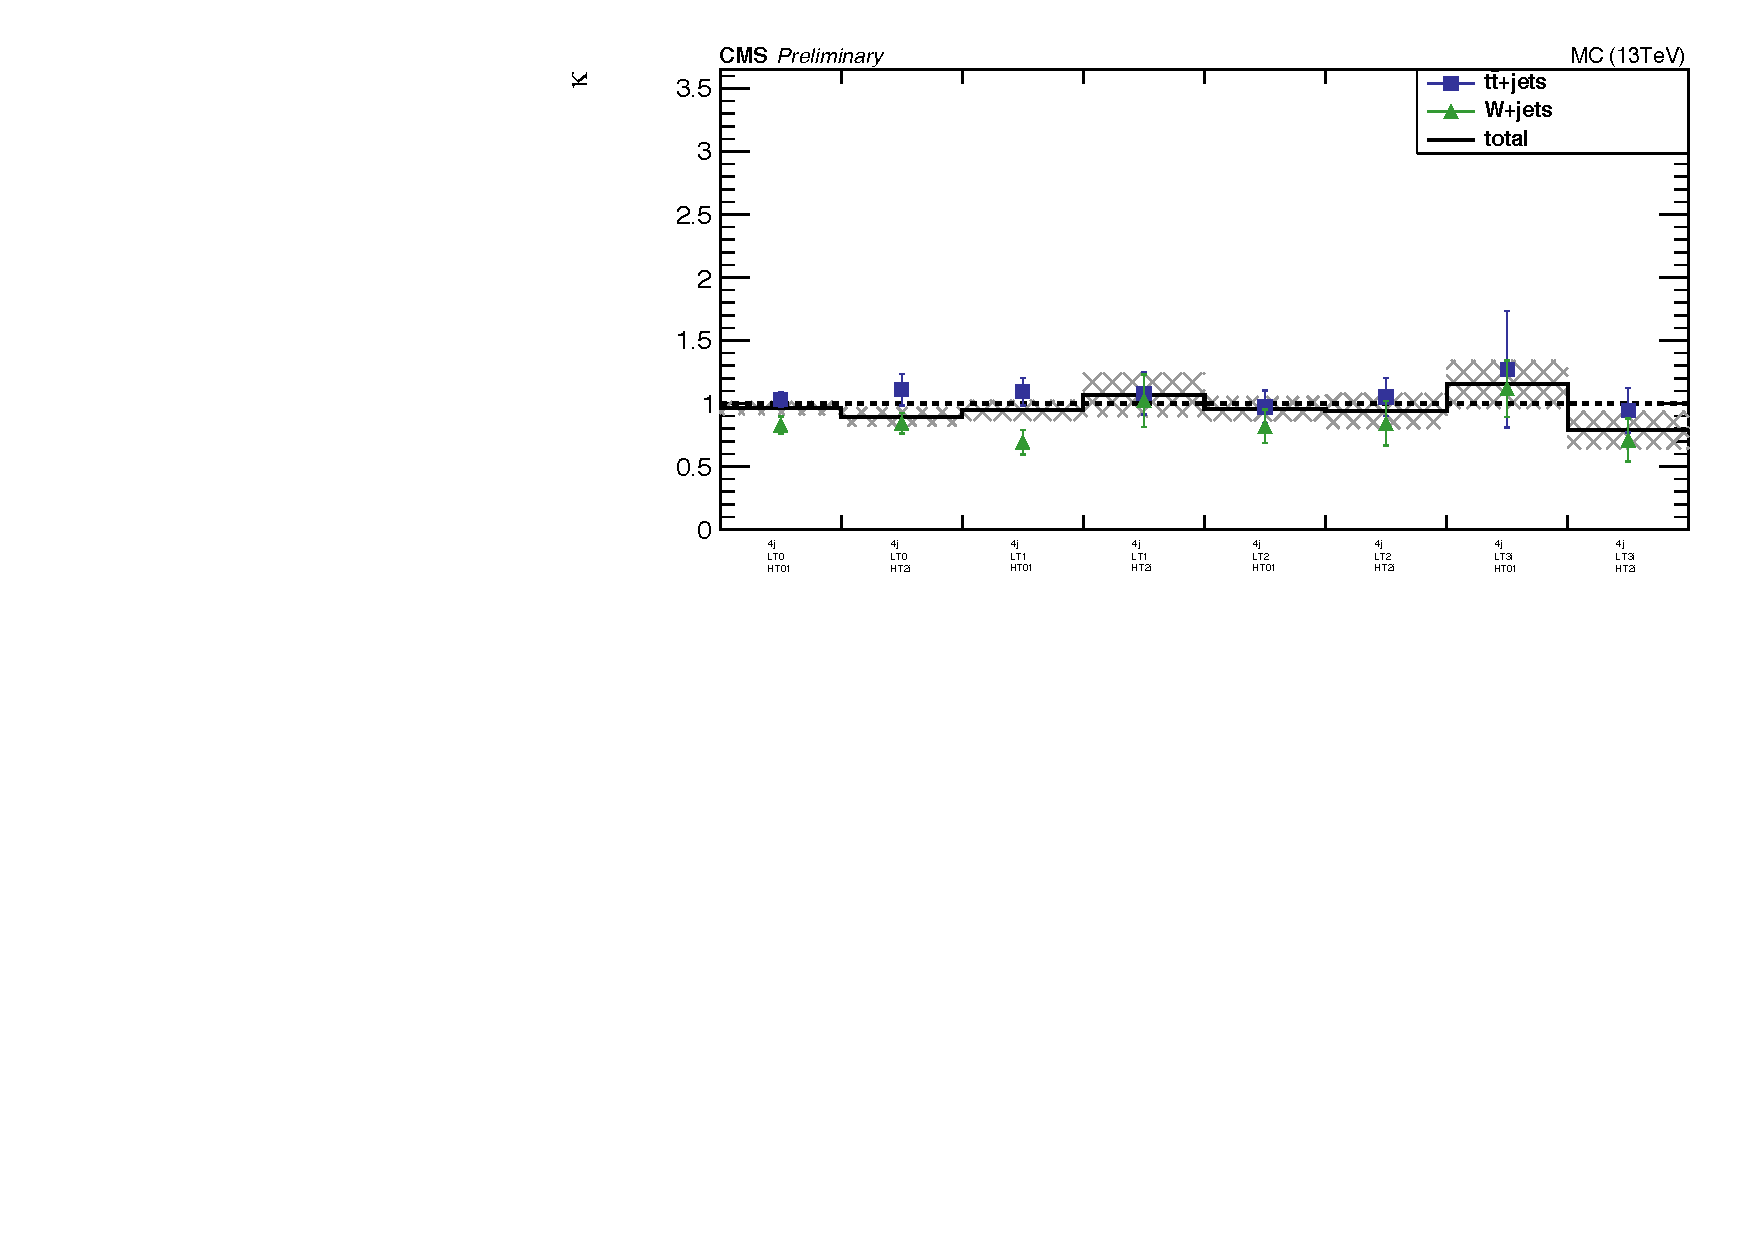
\includegraphics[width=0.8 \textwidth]{Plots/analysis/RCS/Spring16_templates_validation_4j_Moriond2017_lep_data_Kappa}
  \caption[The factors $\kappa_w^{\rm val}$ and the factors $\kappa_{\ttbar}^{\rm val}$ are shown.]{ \label{kappaVal} Correction factors $\kappa_w^{\rm val}$(Green) and $\kappa_{\ttbar}^{\rm val}$(Blue) are shown. The black line represents a $\kappa$, only for illustration, which is the ratio of prediction to the simulation. The shaded area displays the uncertainty from the statistical precision of the simulated samples.}
  \end{center}
\end{figure*}
